\documentclass[11pt]{article}
\usepackage[T1]{fontenc}
\usepackage[utf8]{inputenc}
\usepackage{lmodern}
\usepackage[margin=1.12in]{geometry}
\usepackage{amsmath,amssymb,amsthm,mathtools,mathrsfs}
\usepackage{microtype}
\usepackage{enumitem}
\usepackage{xcolor}
\usepackage{tikz}
\usepackage{hyperref}
\hypersetup{colorlinks=true,linkcolor=blue!45!black,citecolor=blue!45!black,urlcolor=blue!45!black,pdftitle={A Direct Proof of Optimal Max-Cut Hardness},pdfauthor={OpenAI}}
\usepackage[nameinlink,capitalise,noabbrev]{cleveref}
\numberwithin{equation}{section}
\newtheorem{theorem}{Theorem}[section]
\newtheorem{lemma}[theorem]{Lemma}
\newtheorem{proposition}[theorem]{Proposition}
\newtheorem{corollary}[theorem]{Corollary}
\theoremstyle{definition}
\newtheorem{definition}[theorem]{Definition}
\theoremstyle{remark}
\newtheorem{remark}[theorem]{Remark}
\newcommand{\F}{\mathbb F_2}
\newcommand{\E}{\mathbb E}
\newcommand{\one}{\mathbf 1}
\newcommand{\GW}{\alpha_{\mathrm{GW}}}
\DeclareMathOperator{\Aff}{Aff}
\DeclareMathOperator{\Stab}{Stab}
\DeclareMathOperator{\Inf}{Inf}
\DeclareMathOperator{\Val}{Val}
\DeclareMathOperator{\TV}{TV}
\DeclareMathOperator{\supp}{supp}
\DeclareMathOperator{\codim}{codim}
\DeclarePairedDelimiter{\abs}{\lvert}{\rvert}
\DeclarePairedDelimiter{\norm}{\lVert}{\rVert}
\newcommand{\ip}[2]{\langle #1,#2\rangle}
\newcommand{\bits}{\{-1,1\}}
\newcommand{\Bfun}{B}
\newcommand{\cut}{\operatorname{cut}}
\newcommand{\eps}{\varepsilon}
\newcommand{\ind}{\mathbf 1}
\setlist{topsep=4pt,itemsep=2pt}
\allowdisplaybreaks[2]

\title{A Direct Proof of Optimal Max-Cut Hardness}
\author{OpenAI}
\date{September 23, 2026}

\begin{document}
\maketitle
\begin{abstract}
We prove that approximating Max-Cut on simple unweighted graphs within
any fixed factor greater than the Goemans--Williamson constant is NP-hard.
\end{abstract}

\section{Introduction}

For a graph with nonnegative edge weights, Max-Cut asks for a partition of the
vertices maximizing the weight of edges crossing the partition. A cut is
encoded by signs on vertices, and an edge contributes exactly when its signs
differ. For a maximization problem, an $\alpha$-approximation returns a
feasible solution worth at least $\alpha$ times the optimum. Unless stated
otherwise, the graph and its rational weights are given explicitly.
We write $\operatorname{MaxCut}(G)$ for the maximum crossing weight and,
when the edge weights sum to one, also denote this value by $\Val(G)$.
The decision problem of whether a weighted graph has a cut of at least a
given weight appears among Karp's original NP-complete
problems~\cite{Karp72}. Approximation asks how much of this optimum can
still be guaranteed in polynomial time.
Goemans and Williamson~\cite{GW95} gave a semidefinite programming algorithm with random-hyperplane rounding
for Max-Cut, with expected approximation ratio approaching
\begin{equation}\label{eq:gw-constant}
 \GW=\min_{-1\le \rho<1}
 \frac{2\arccos\rho}{\pi(1-\rho)}
 =0.878567\ldots.
\end{equation}
The expression compares two contributions of an edge whose endpoint
vectors have inner product $\rho$: its semidefinite objective value is
$(1-\rho)/2$, whereas a random hyperplane separates the vectors with
probability $\arccos(\rho)/\pi$. The minimum ratio over $\rho$ is the
uniform guarantee of this rounding rule.
Determining whether this ratio is optimal under ordinary NP-hardness has
been a central question in approximation algorithms. H\aa stad's
hardness theorem~\cite{Hastad01}, combined with the gadgets of
Trevisan, Sorkin, Sudan, and Williamson~\cite{TSSW00}, rules out ratios
greater than $16/17$.
Khot, Kindler, Mossel, and O'Donnell~\cite{KKMO07} established optimality of
$\GW$ assuming the Unique Games Conjecture~\cite{Khot02}; the analytic input
is the Majority Is Stablest theorem of Mossel, O'Donnell, and
Oleszkiewicz~\cite{MOO10}.

We resolve the unconditional optimality question for Max-Cut.

\begin{theorem}\label{thm:main}
For every fixed $\alpha$ with $\GW<\alpha\le1$, it is NP-hard to approximate
Max-Cut within a factor of $\alpha$. This holds for simple unweighted graphs.
\end{theorem}

The statement means that a polynomial-time algorithm which always returns a
cut of weight at least $\alpha$ times the maximum would imply
$\mathrm P=\mathrm{NP}$. We prove the following more precise gap theorem.
Write
\begin{equation}\label{eq:B}
 B(t)=\frac{2}{\pi}\arcsin t,\qquad 0<t<1.
\end{equation}

\begin{theorem}\label{thm:gap}
Fix a rational $t\in(0,1)$ and a constant
$0<\eps<(t-B(t))/4$. For graphs equipped with a rational probability
distribution on edges, it is NP-hard to distinguish
\begin{align*}
 \textnormal{YES:}\quad&\Val\ge\frac{1+t}{2}-\eps,\\
 \textnormal{NO:}\quad&\Val\le\frac{1+B(t)}{2}+\eps,
\end{align*}
where $\Val$ is the maximum cut weight.
\end{theorem}

\subsection*{Prior work and the direct route}

The reduction of proof verification to approximation gaps has its roots in
Feige, Goldwasser, Lov\'asz, Safra, and Szegedy~\cite{FGLSS96} and in the
PCP theorems of Arora--Safra and Arora, Lund, Motwani, Sudan, and
Szegedy~\cite{AroraSafra98,ALMSS98}. H\aa stad's Fourier analysis of
proof-verification tests~\cite{Hastad01} made many of these gaps sharp.
For Max-Cut, the Gaussian geometry of the semidefinite relaxation gives
a particularly precise target. Feige and Schechtman~\cite{FS02}
constructed integrality gaps approaching $\GW$ for this relaxation;
a limitation of that relaxation alone does not establish hardness for
arbitrary algorithms. The Unique Games reduction of
Khot, Kindler, Mossel, and O'Donnell~\cite{KKMO07} connected the same
geometric threshold to computational hardness.

The original analysis of Khot, Kindler, Mossel, and O'Donnell proposed
Majority Is Stablest as the analytic statement needed to obtain this
threshold. Mossel, O'Donnell, and Oleszkiewicz proved it through a
comparison between low-influence Boolean functions and Gaussian
functions~\cite{MOO10}, transferring Borell's halfspace noise-stability
bound~\cite{Borell85} to the Boolean setting. Their theorem leaves the
Unique Games Conjecture as the hypothesis in the classical hardness
reduction~\cite[Corollary~2.12]{MOO10}. We use Majority Is Stablest to
identify an influential coordinate of our test, then prove the additional
extraction needed to turn that coordinate into a source-game label.
The algorithmic benchmark above is the ideal rounding ratio;
finite-precision SDP optimization and random-hyperplane rounding give
expected ratio $\GW-\eta$ for any fixed $\eta>0$~\cite[Section~2]{GW95}.

The comparison between semidefinite approximation and hardness extends
beyond a single worst-case ratio. O'Donnell and Wu~\cite{OW08}
determined the full Max-Cut approximation curve under the Unique Games
Conjecture, relating the attainable cut value to the instance's optimum.
Raghavendra~\cite{Raghavendra08} established a general correspondence
between semidefinite relaxations and Unique-Games-based hardness for
finite constraint satisfaction problems. Our theorem concerns the
unconditional worst-case ratio for Max-Cut; the proof below establishes
the specific family of completeness and soundness gaps in
\Cref{thm:gap}.

In a projection game, each vertex of a bipartite graph receives a label
from a specified alphabet, and the edge weights form a probability
distribution. An edge accepts when its prescribed map sends the left label to the
right label. Its value is the maximum accepted edge weight. A two-to-one
constraint has exactly two preimages for every right label. Completeness
and soundness are, respectively, the promised lower bound on the YES-case
value and upper bound on the NO-case value.

Our starting point is the published 2-to-1 game construction with imperfect
completeness~\cite{DKKMS25}. The Grassmann-graph approach was introduced
by Khot, Minzer, and Safra~\cite{KMS25}. Its soundness was completed
through the connection between expansion and agreement established by
Barak, Kothari, and Steurer~\cite{BKS19} and the expansion theorem of
Khot, Minzer, and Safra~\cite{KMS23}. We need a precise affine form of the
construction: its projections are surjective affine maps between binary
spaces of dimensions differing by one, and its alphabet can be fixed for a
desired soundness before the completeness error is made arbitrarily small.
\Cref{prop:affine-games} states this input. Appendix~\ref{sec:affine-games}
derives it from the published construction, specifying both the
valid-subspace conditioning and the auxiliary candidate lists used in
the soundness proof.
Together with Majority Is Stablest, that construction supplies the
external foundation of the argument. The Unique Games Conjecture enters
only as historical context. The tree Fourier analysis, hashing bound,
and hidden-coordinate decoding are proved here.

\subsection*{The proof and its main ingredients}

As in long-code reductions~\cite{BGS98,Hastad01}, a label $a$ is represented
by the dictator $w\mapsto w(a)$, where $w$ ranges over Boolean words
indexed by labels. The graph has one such word domain for each tuple of
left vertices of the source game. Thus an arbitrary cut specifies a
Boolean function on each domain. To sample an edge, the test chooses two
left tuples through a common right tuple, generates two words on the
right label space, and pulls them back through the sampled affine
projections. It negates the second word. When the sampled constraints
are satisfied, dictator labels give a cut probability of one half of one
plus the correlation between the two words evaluated at a common label.

The word generator is a finite rooted tree. Every internal node has $s$
pairs of children and a random table from $\F^s$ to $\bits$; the leaves
carry affine forms on the label space. At a label $a$, these forms give
leaf signs, and the tables recursively combine the child signs into the
root sign $W(a)$. The gate rule is chosen so that each monomial of its
Walsh expansion keeps one child from every pair. A second exploration
keeps both children of one randomly selected pair at each reached node.
At any fixed depth, the two explorations have exactly one node in
common. The test couples the tables reached by this second exploration
at a random depth, using entrywise correlation $t$, and leaves all other
tables unchanged. Every monomial therefore acquires precisely one factor
of $t$. A small independent resampling of the affine rows gives the
smoothing needed for soundness and only a small completeness loss.

For an arbitrary cut, we first average its odd part over the source-game
edges. The resulting function is balanced in the selected table entries,
and a cut above the desired NO threshold makes its expected noise
stability exceed $B(t)$. Majority Is Stablest then detects an influential
entry. That entry is indexed by a gate input, not by a source-game label.
The remaining task is to connect its influence to labels that the two
endpoints of a source edge can choose consistently. Three steps address
this task.

\begin{enumerate}
\item \emph{Local simplification of Fourier support.}
The gate symmetries force the two child indices in each pair to have the
same sum. After row smoothing, averaging the depth of the selected tables
makes it inexpensive to retain indices which put this sum in one child of
each pair and zero in the other. This simplification is imposed only at
the influential gate. It is the structure that lets affine shifts act as
translations of that gate's table.

\item \emph{A vector-valued affine hashing lemma.}
For independent affine shifts, a diffuse distribution of Fourier mass
cannot create a large entry influence on average. The bound is uniform in
the dimension of the row space. Its proof uses two truncations and a
fourth-moment identity; it may be useful whenever translated coefficient
arrays must be decoded without an alphabet-size loss.

\item \emph{Decoding with a hidden coordinate.}
The mass concentration is obtained after fixing many row coordinates.
A left endpoint cannot usually construct the pullback of this context
without knowing its incident projection. We use a product of the game
and plant zero linear coefficients in one uniformly chosen factor of
the context and of the latent resampling rows. After that factor is
forgotten, the planted law is close to the original law. At the planted
factor, the context can be pulled back without knowing the projection.
Only the $2s$ free rows at the selected gate still have to be compared
across it, at a cost of $2^{2s}$ in Fourier mass.
\end{enumerate}

The resulting decoding loss is independent of the source alphabet.
This is essential: the alphabet dimension depends on the soundness we
request, so a dimension-dependent loss could make the soundness choice
circular. We first fix that loss and the source soundness, then the
alphabet and the number of product factors, and finally the source
completeness error. The quantifier order in
\Cref{prop:affine-games} permits exactly this sequence.

\Cref{sec:preliminaries} fixes the Fourier conventions.
\Cref{sec:tree,sec:reduction} define the code and the Max-Cut test.
\Cref{sec:tree-fourier,sec:hashing,sec:extraction} prove the analytic ingredients.
\Cref{sec:decoding,sec:completion} give the decoding and finish the proof.
Appendix~\ref{sec:affine-games} derives the precise starting game from the
published construction, and Appendix~\ref{sec:unweighted} gives a deterministic
conversion to simple unweighted graphs.

\section{Preliminaries}\label{sec:preliminaries}

The proof uses two Fourier expansions. Characters of affine rows encode
candidate labels, whereas characters of Boolean table entries detect the
influences to which Majority Is Stablest applies. We introduce both
conventions, then state the exact affine-game input.

All vector spaces over $\F$ are finite dimensional. All expectations on a
finite vector space or Boolean cube use the uniform probability measure,
unless another distribution is specified. All Fourier coefficients use
this probability normalization. An $L^2$ norm always integrates over the
variables displayed in its subscript; variables declared fixed are not
integrated.

\subsection{Affine rows and labels}

Let $\mathcal A$ be a nonempty affine space over $\F$, with a fixed affine
coordinate system, and set
\[
 H=\Aff(\mathcal A,\F).
\]
This is a vector space, containing the constant form $\one$.
For $q\in H^*$ define $\chi_q(h)=(-1)^{q(h)}$.
Evaluation identifies $\mathcal A$ with
\begin{equation}\label{eq:labels-dual}
 \{q\in H^*:q(\one)=1\}.
\end{equation}
Indeed, if $h(a)=h_0+\sum_i h_i a_i$, a functional taking value one on
$\one$ has the unique form $q(h)=h_0+\sum_i h_i a_i$.
We call precisely these functionals \emph{labels}; a general nonzero
functional in $H^*$ need not be a label.

For $f:H^k\to\mathbb R$ and $C=(q_1,\ldots,q_k)\in(H^*)^k$, put
\[
 \widehat f(C)=\E_R f(R)\prod_{i=1}^k\chi_{q_i}(R_i),\qquad
 |C|=\#\{i:q_i\ne0\}.
\]
Parseval gives $\sum_C\widehat f(C)^2=\E_R f(R)^2$.
The same notation is used for functions with additional variables, which
remain fixed during the indicated Fourier expansion.

For $0\le r\le1$, let $T_r$ be the row-noise operator: independently in each
coordinate, retain the row with probability $r$ and otherwise replace it
by an independent uniform row. Then
\begin{equation}\label{eq:row-noise}
 \widehat{T_rf}(C)=r^{|C|}\widehat f(C).
\end{equation}
This operator preserves the range $[-1,1]$. It is also convolution by an
independent increment $E\in H^k$, whose coordinates are zero with
probability $r$ and independent uniform rows with probability $1-r$.
Convolution commutes with every fixed translation of the rows.

\subsection{Boolean Fourier analysis}

For a finite set $\Omega$ and $h:\bits^\Omega\to\mathbb R$, write
\[
 h(x)=\sum_{S\subseteq\Omega}\widehat h(S)\prod_{a\in S}x_a.
\]
Its influence and degree-$K$ influence at $a\in\Omega$ are
\[
 \Inf_a(h)=\sum_{S\ni a}\widehat h(S)^2,\qquad
 \Inf_a^{\le K}(h)=\sum_{\substack{S\ni a\\|S|\le K}}
 \widehat h(S)^2.
\]
Let $P_{\le K}$ be the orthogonal projection onto Fourier degree at most
$K$. In particular,
\begin{equation}\label{eq:degree-influence}
 \sum_{a\in\Omega}\Inf_a(P_{\le K}h)
 \le K\norm{h}_2^2.
\end{equation}
For $t$-correlated uniform bits $x,y$, independently coupled in each
coordinate,
\begin{equation}\label{eq:stability}
 \Stab_t(h)=\E[h(x)h(y)]
 =\sum_{S\subseteq\Omega}t^{|S|}\widehat h(S)^2.
\end{equation}
Thus stability is nonnegative for $t\ge0$. If $h\in[-1,1]$, it is at most
one.

\begin{lemma}[Majority Is Stablest with a degree cutoff]\label{lem:mis}
Fix $0<t<1$ and $\xi>0$. There are an integer $K\ge1$ and $\tau>0$,
depending only on $t,\xi$, such that every
$h:\bits^\Omega\to[-1,1]$ with $\E h=0$ satisfies
\[
 \bigl(\Inf_a^{\le K}(h)<\tau\text{ for all }a\in\Omega\bigr)
 \quad\Longrightarrow\quad
 \Stab_t(h)\le B(t)+\xi.
\]
\end{lemma}

\begin{proof}
The untruncated assertion follows from Majority Is Stablest
\cite[Theorem~4.4]{MOO10}. To match its $[0,1]$ convention, put
$g=(h+1)/2$: then $\E g=1/2$, each nonconstant Fourier coefficient is
halved, and $\Stab_t(h)=4\Stab_t(g)-1$. The Gaussian halfspace value
for $g$ is $1/4+\arcsin(t)/(2\pi)$, which becomes $B(t)$ in our
normalization; see \cite[Theorem~4.1 and Corollary~4.3]{MOO10} and
\cite{Borell85}. Here is the degree-cutoff reduction to the untruncated
assertion. For a cube-noise
parameter $u<1$, put $h_u=T_u h$, using ordinary bit noise in this
paragraph. Range and mean are preserved. Uniformly over $h$ of norm at
most one,
\[
 0\le\Stab_t(h)-\Stab_t(h_u)
 \le\sup_{j\ge0}t^j(1-u^{2j})\longrightarrow0
 \quad(u\uparrow1).
\]
The convergence follows by first choosing a finite degree cutoff to bound
the tail $t^j$, and then taking $u$ close to one on the remaining degrees.
Choose $u$ so that this error is at most $\xi/2$. Let $\delta>0$ be the
untruncated influence threshold for error $\xi/2$. Choose $K$ with
$u^{2(K+1)}\le\delta/2$, and take $\tau=\delta/2$. Then
\[
 \Inf_a(h_u)
 \le\Inf_a^{\le K}(h)+u^{2(K+1)}\norm{h}_2^2
 <\delta.
\]
Apply the untruncated theorem to $h_u$ and add the stability error.
\end{proof}

\subsection{Affine projection games}

A weighted bipartite projection game consists of finite sets $X,Y$, a
rational probability distribution $\lambda$ on a finite edge set
$E$ with endpoint maps to $X$ and $Y$ (parallel edges are allowed), finite alphabets,
and a projection $\pi_e$ for each edge. Its value is
\[
 \Val(\mathcal G)=
 \max_{\ell_X,\ell_Y}\Pr_{e=(x,y)\sim\lambda}
 [\pi_e(\ell_X(x))=\ell_Y(y)].
\]
In this paper the alphabets are $\F^{n+1}$ and $\F^n$, and every
$\pi_e:\F^{n+1}\to\F^n$ is surjective affine.
\Cref{prop:affine-games} supplies NP-hard gaps with this structure.
We discard endpoints with zero marginal probability whenever conditional
edge distributions are used.

The starting theorem has the quantifier order
\[
 \forall b\in(0,1)\quad \exists n=n(b)\ge1\quad
 \forall a\in(0,1-b).
\]
The precise promise is given below; its derivation from
the published construction is in \Cref{sec:affine-games}.

\begin{proposition}[Affine 2-to-1 Games Theorem]
\label{prop:affine-games}
For every constant $b\in(0,1)$ there is an integer $n\geq 1$ such that,
for every constant $a\in(0,1-b)$, the following promise problem is NP-hard.
Its input is a
weighted bipartite game with vertex sets $X,Y$, respective label sets
$\F^{n+1},\F^n$, and a surjective affine map
\[
  \pi_e:\F^{n+1}\longrightarrow\F^n
\]
on each edge $e=(x,y)$.  An edge is satisfied when
$\pi_e(\lambda_X(x))=\lambda_Y(y)$.  The promise cases are
\[
  \mathrm{YES}:\quad \Val(\mathcal G)\geq 1-a,
  \qquad
  \mathrm{NO}:\quad \Val(\mathcal G)\leq b.
\]
The integer $n$ depends on $b$ alone.  For fixed $a,b$, the reduction is
deterministic and has polynomial running time and output size.
\end{proposition}

A weighted graph is likewise specified by a rational distribution on
unordered edges, allowing loops. A cut assigns signs to its vertices and
satisfies an edge when its signs differ. Its value is its satisfaction
probability. Loops have zero cut weight. The conversion in
\Cref{lem:unweighted} keeps a common scale even when loops are deleted.

\section{A tree code with complementary traversals}
\label{sec:tree}

We use the affine label space $\mathcal A$ and row space
$H=\Aff(\mathcal A,\F)$ of \Cref{sec:preliminaries}.
The code below turns affine rows and Boolean gate tables into a word
indexed by labels. Its two complementary traversals control the
correlation seen by a cut that evaluates the word at a single label.

\begin{definition}[Tree code]
\label{def:tree-code}
Fix integers $s\ge2$ and $m\ge1$, and put
\[
 k=(2s)^m,\qquad d=s^m.
\]
Let $\mathcal T$ be the complete rooted $2s$-ary tree of depth $m$.
The children of each internal node $v$ are indexed by
$(g,b)\in[s]\times\{0,1\}$.  Its leaves are indexed by $[k]$.
To each internal node assign a table
$F_v:\F^s\to\{-1,1\}$, and to each leaf assign a row $R_i\in H$.
The word $W(R,F)\in\{-1,1\}^{\mathcal A}$ is defined pointwise as
follows.  At $a\in\mathcal A$, leaf $i$ has sign $(-1)^{R_i(a)}$.
An internal node with child signs $(Z_{g,b})$ outputs
\begin{equation}
 \left(\prod_{g=1}^s Z_{g,0}\right)F_v(z),
 \qquad (-1)^{z_g}=Z_{g,0}Z_{g,1}.
 \label{eq:gate-rule}
\end{equation}
The root output is $W(R,F)(a)$.
\end{definition}

We choose the tables to be noised by a second traversal of the tree.
A \emph{random slice} is obtained by first choosing
$J_0$ uniformly from $\{0,\ldots,m-1\}$.  Starting at the root,
at each reached node of depth less than $J_0$ choose one of its $s$
child pairs uniformly and independently, and continue through both
children of that pair.  The set $\mathcal D$ of reached nodes at
depth $J_0$ is the slice.

Conditionally on $J_0=j$, the slice has $2^j$ nodes, and every fixed
node of depth $j$ belongs to it with probability $s^{-j}$.
We write $F_{\rm out}=(F_u)_{u\notin\mathcal D}$ for the tables
outside the slice.

The two traversals of the tree used below complement one another.
The slice construction chooses one pair and keeps both children.
The Walsh expansion of a gate keeps one child from every pair.
Their intersection therefore follows a single path. Figure~\ref{fig:traversals}
shows the local rule; iterating it gives one common node at every slice depth.

\begin{figure}[ht]
\centering
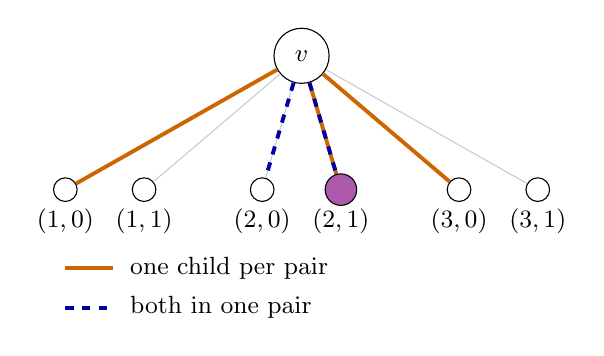
\begin{tikzpicture}[x=1cm,y=1cm,every node/.style={font=\small},
  mono/.style={draw=orange!80!black,line width=1.4pt},
  slice/.style={draw=blue!65!black,line width=1.4pt,dashed}]
\node[circle,draw,minimum size=7mm] (v) at (0,1.7) {$v$};
\foreach \x/\name/\lab in {-3/a/{(1,0)},-2/b/{(1,1)},-.5/c/{(2,0)},.5/d/{(2,1)},2/e/{(3,0)},3/f/{(3,1)}} {
 \node[circle,draw,fill=white,minimum size=3mm,inner sep=1pt] (\name) at (\x,0) {};
 \node[below] at (\x,-.12) {$\lab$};
 \draw[gray!40] (v) -- (\name);
}
\draw[mono] (v) -- (a);
\draw[mono] (v) -- (d);
\draw[mono] (v) -- (e);
\draw[slice] (v) -- (c);
\draw[slice] (v) -- (d);
\node[circle,draw,fill=violet!65,minimum size=4mm,inner sep=1pt] at (.5,0) {};
\draw[mono] (-3,-1) -- (-2.4,-1);
\node[anchor=west] at (-2.3,-1) {one child per pair};
\draw[slice] (-3,-1.5) -- (-2.4,-1.5);
\node[anchor=west] at (-2.3,-1.5) {both in one pair};
\end{tikzpicture}

\caption{Complementary choices at one gate, illustrated for $s=3$.
A monomial traversal (solid) selects one child from each pair; the slice
exploration (dashed) selects both children of one pair. Exactly one child
is shared, shown in purple. Only this local selection is depicted;
the same rule is repeated above the chosen slice.}
\label{fig:traversals}
\end{figure}

\begin{lemma}[Complementary traversal and correlation]
\label{lem:tree-correlation}
For every fixed collection of tables $F$, the root output as a
multilinear polynomial in the $k$ leaf signs has only degree-$d$
monomials.  Each such monomial chooses one child from every pair
at every node that it reaches.  Every resulting traversal meets
every possible slice $\mathcal D$ at exactly one node.
Consequently, negating all the tables on a slice negates $W$.

Let $0<t<1$ and $0<r<1$.  Draw $F$ uniformly, and construct $F'$
by leaving the tables outside $\mathcal D$ unchanged and coupling
each pair of corresponding table entries on $\mathcal D$ as
uniform signs of correlation $t$, independently across entries.
Independently draw
$R\in H^k$ uniformly, and form $R^1,R^2$ by retaining each row of
$R$ with probability $r$ and otherwise replacing it by an
independent uniform row, independently in the two copies.
Then, for every $a\in\mathcal A$ and every fixed slice,
\begin{equation}
 \E\bigl[W(R^1,F)(a)W(R^2,F')(a)\mid\mathcal D\bigr]
       =t r^{2d}.
 \label{eq:tree-correlation}
\end{equation}
In particular, if $r=1-\mu/d$ with $0<\mu<1/2$, then
$r^{2d}\ge1-2\mu$.
\end{lemma}

\begin{proof}
For a fixed gate table, expand in its argument $z$:
$F_v(z)=\sum_{I\subseteq[s]}\widehat F_v(I)(-1)^{\sum_{g\in I}z_g}$.
Substituting into Equation~\eqref{eq:gate-rule}, the term indexed
by $I$ is
\[
 \widehat F_v(I)
 \prod_{g\notin I}Z_{g,0}\prod_{g\in I}Z_{g,1}.
\]
Iterating this expansion gives
\begin{equation}
 W_F(x)=\sum_{P\in\mathscr P}a_P(F)\prod_{i\in P}x_i,
 \qquad |P|=d,
 \label{eq:tree-polynomial}
\end{equation}
where $\mathscr P$ is the family of leaf sets produced by choosing
one child per pair at each reached internal node.  The leaf set
determines all these choices: a selected child has a nonempty
intersection with that leaf set, whereas an unselected child has
none.  Thus different traversals give different monomials, and
$a_P(F)$ is the product of one Walsh coefficient of $F_v$ for each
node reached by the traversal.

At the root both a monomial traversal and the slice exploration
are present.  At any common node above the slice depth, exactly
one child is selected by both explorations.  Induction gives
exactly one common node at the slice depth.  Hence each $a_P$
contains exactly one factor from a table on $\mathcal D$.
Negating every such table negates each coefficient in
Equation~\eqref{eq:tree-polynomial} and therefore negates the word.
Moreover, each Walsh coefficient of a slice table satisfies
\[
 \E[\widehat F'_v(I)\mid F_v]=t\widehat F_v(I).
\]
Conditional independence between tables therefore gives
$\E[a_P(F')\mid F,\mathcal D]=t a_P(F)$.

For fixed $a$, the signs
$x_i^b=(-1)^{R_i^b(a)}$ are uniform, independent across $i$, and
$\E[x_i^1x_i^2]=r^2$.  Thus the product expectation of two
monomials in Equation~\eqref{eq:tree-polynomial} is zero unless
their leaf sets agree, and is $r^{2d}$ when they agree.
Since $W_F$ is Boolean, Parseval gives $\sum_P a_P(F)^2=1$.
Averaging first over rows and then over $F'$ proves
Equation~\eqref{eq:tree-correlation}.  The last claim is
Bernoulli's inequality:
$(1-\mu/d)^{2d}\ge1-2\mu$.
\end{proof}

The correlation identity describes a cut that evaluates the word at
one label. To analyze arbitrary cuts, we also need functions that can
depend on the entire word but do not see its generating rows or tables.
We call $f$ a \emph{function of the code} if
\begin{equation}
 f(R,F)=\phi(W(R,F))
 \label{eq:function-of-code}
\end{equation}
for a fixed function $\phi$ on words.  This class is closed under
averaging over fixed choices of $\phi$, including choices that
first pull a word back through a fixed affine map.
For $r\in[0,1]$, let $T_r$ denote independent row resampling with
retention probability $r$, and write $\bar f=T_rf$.
The operator preserves bounds on the range of $f$.
If $\phi$ is odd, Lemma~\ref{lem:tree-correlation} shows that both
$f$ and $\bar f$ are odd under simultaneous negation of the slice
tables.  In particular, they have mean zero in those table entries
when all rows and outside tables are fixed.

At these fixed data, the remaining random input is the cube of
$|\mathcal D|2^s$ independent entries, indexed by
$(v,z)\in\mathcal D\times\F^s$. Fourier degree and influence on this
cube refer to subsets of \emph{entries}. This differs from the Walsh
expansion of a fixed gate in its $s$-bit argument $z$ used in the
correlation proof.

\section{The Max-Cut reduction}\label{sec:reduction}

Fix a rational $t\in(0,1)$, tree parameters $s,m$, a rational
$0<\mu<1/2$, and $r=1-\mu/d$. The parameters will be chosen in
\Cref{sec:completion}. Let $\mathcal G$ be an affine game as in
\Cref{prop:affine-games}, with edge law $\lambda$ and alphabet dimensions
$n+1,n$. Let $T\ge1$ be an integer. We use the product label spaces
\[
 \mathcal B=(\F^{n+1})^T,\qquad
 \mathcal A=(\F^n)^T,
\]
and the row space $H=\Aff(\mathcal A,\F)$.

\subsection{Vertices and edge distribution}

For each $\underline x\in X^T$, make one graph vertex
$(\underline x,w)$ for every word $w\in\bits^{\mathcal B}$.
This is the standard long-code word domain~\cite{BGS98,Hastad01};
the tree construction specifies how the test samples its queries.
Thus an arbitrary cut is exactly a family of functions
\[
 \sigma_{\underline x}:\bits^{\mathcal B}\longrightarrow\bits.
\]
The functions receive only the resulting words; they do not receive the
rows, gate tables, slice, or sampled game edges that produced them.

The graph's edge distribution is the following test.
\begin{enumerate}
\item Draw $\underline y\in Y^T$ from the product right-endpoint marginal
of $\lambda$. Independently draw two edge tuples
$\underline e,\underline e'$ from the product conditional edge law given
$\underline y$. Write $\underline x,\underline x'$ for their left
endpoints and
$\pi_{\underline e},\pi_{\underline e'}:\mathcal B\to\mathcal A$
for their coordinatewise projections.

\item Independently of all game data, draw a random slice $\mathcal D$.
Draw $F,F'$ as in \Cref{lem:tree-correlation}: corresponding entries
are independent $t$-correlated uniform pairs on $\mathcal D$, and
identical uniform pairs off $\mathcal D$.

\item Draw a uniform common row array $R\in H^k$. In each of two copies,
independently retain each row with probability $r$ and otherwise resample
it uniformly, obtaining $R^1,R^2$.

\item Output the unordered edge whose endpoints are
\begin{equation}\label{eq:test-queries}
 \bigl(\underline x,W(R^1,F)\circ\pi_{\underline e}\bigr),
 \qquad
 \bigl(\underline x',-W(R^2,F')\circ\pi_{\underline e'}\bigr).
\end{equation}
\end{enumerate}
All edge weights are the probabilities of these outcomes, aggregated over
outcomes with the same unordered endpoints.

\begin{lemma}[Completeness]\label{lem:completeness}
If $\Val(\mathcal G)\ge1-a$, the graph has a cut of value at least
\begin{equation}\label{eq:completeness}
 (1-2Ta)\frac{1+t r^{2d}}2
 \ge\frac{1+t}{2}-t\mu-2Ta.
\end{equation}
The first lower bound is useful when $2Ta\le1$, which is the regime used
below.
\end{lemma}

\begin{proof}
Choose game labels $\ell_X,\ell_Y$ satisfying an edge with probability at
least $1-a$. Label each word vertex by evaluation at the tuple of left
labels:
\[
 \sigma_{\underline x}(w)=
 w\bigl(\ell_X(x_1),\ldots,\ell_X(x_T)\bigr).
\]
Each coordinate of either sampled edge tuple has the original edge law.
A union bound shows that all $2T$ sampled constraints are satisfied except
with probability at most $2Ta$. When all these constraints are satisfied,
the two queried tuples
project to the same label
$l=(\ell_Y(y_1),\ldots,\ell_Y(y_T))\in\mathcal A$.
The cut signs then have product
$-W(R^1,F)(l)W(R^2,F')(l)$. The word-generation data are independent of
the game edges, so \Cref{lem:tree-correlation} gives conditional cut
probability $(1+t r^{2d})/2$. On the remaining event the cut probability
is nonnegative. This proves the first bound when $2Ta\le1$; if $2Ta>1$
that bound is negative and is automatic. Finally,
$r^{2d}\ge1-2\mu$, and the loss due to the prefactor is at most $2Ta$,
giving the second bound.
\end{proof}

\subsection{A large cut produces excess stability}

An arbitrary cut need not change sign when its queried word is negated.
We separate its two parities because the negative second query makes
odd dependence increase the cut value and even dependence decrease it.
For each cut table define its even and odd parts by
\[
 \sigma^{\mathrm{even}}(w)=\frac{\sigma(w)+\sigma(-w)}2,
 \qquad
 \sigma^o(w)=\frac{\sigma(w)-\sigma(-w)}2.
\]
For an edge tuple and a right-endpoint tuple, set
\begin{align}
 G_{\underline e}(R,F)
 &=\sigma^o_{\underline x(\underline e)}
       (W(R,F)\circ\pi_{\underline e}),\label{eq:edge-function}\\
 G_{\underline y}(R,F)
 &=\E_{\underline e\mid\underline y}G_{\underline e}(R,F),
 \qquad \bar G_{\underline y}=T_rG_{\underline y}.
 \label{eq:average-function}
\end{align}
Write $A_{\underline y}$ and $\bar A_{\underline y}=T_rA_{\underline y}$
for the analogous averages using $\sigma^{\mathrm{even}}$.
These functions are bounded in absolute value by one.
Moreover,
\[
 G_{\underline y}(R,F)=\phi_{\underline y}(W(R,F)),\qquad
 \phi_{\underline y}(w)=\E_{\underline e\mid\underline y}
 \sigma^o_{\underline x(\underline e)}(w\circ\pi_{\underline e}),
\]
where $\phi_{\underline y}$ is odd and depends on no slice or row data.
Thus $\bar G_{\underline y}$ has mean zero in the slice entries for
every fixed $\underline y,\mathcal D,R,F_{\mathrm{out}}$, by the
observation following \Cref{lem:tree-correlation}.
The later extraction argument, \Cref{prop:extraction}, applies to precisely
such bounded odd functions of the generated word.

\begin{lemma}[Stability identity]\label{lem:cut-stability}
For every cut of the constructed graph,
\begin{equation}\label{eq:cut-stability}
 \cut(\sigma)=\frac12+
 \frac12\E\Stab_t^{F_{\mathcal D}}(\bar G_{\underline y})
 -\frac12\E\Stab_t^{F_{\mathcal D}}(\bar A_{\underline y}),
\end{equation}
where both expectations are over
$\underline y,\mathcal D,R,F_{\mathrm{out}}$.
In particular,
\begin{equation}\label{eq:cut-upper-stability}
 \cut(\sigma)\le\frac12+
 \frac12\E\Stab_t^{F_{\mathcal D}}(\bar G_{\underline y}).
\end{equation}
\end{lemma}

\begin{proof}
Condition on $\underline y,\mathcal D,R,F_{\mathrm{out}}$.
The sampled edge tuples and the two row resamplings are independent
between copies. After averaging over them, the expected first sign as a
function of $F_{\mathcal D}$ is $\bar A_{\underline y}+\bar G_{\underline y}$.
The minus sign in the second queried word makes the expected second sign
$\bar A_{\underline y}-\bar G_{\underline y}$ at $F'_{\mathcal D}$.
The two slice inputs are ordinary $t$-correlated uniform cube inputs.
The rows in these functions are the common latent array $R$; the two
independent row resamplings have already been absorbed into $T_r$.
Negating every slice entry leaves $\bar A_{\underline y}$ unchanged and
negates $\bar G_{\underline y}$. Their Fourier supports therefore have
opposite total parities, so the cross terms vanish. The expected sign
product is
$\Stab_t(\bar A_{\underline y})-\Stab_t(\bar G_{\underline y})$.
An edge is cut with probability one half of one minus its sign product,
giving \eqref{eq:cut-stability}. Nonnegativity of stability for $t>0$
gives \eqref{eq:cut-upper-stability}.
\end{proof}

If a cut has value at least $(1+B(t))/2+\delta/2$, then its odd average
has expected slice stability at least $B(t)+\delta$.
The next three sections show that this excess stability yields a label
carrying substantial Fourier mass, with constants independent of the game
dimension and the number of repetitions; the formal statement is
\Cref{prop:extraction}. \Cref{sec:decoding} then turns that mass into a
labeling of a single copy of the original game.

\section{Fourier structure of the tree code}\label{sec:tree-fourier}

The cut depends on the generated word, so every transformation that
preserves that word also constrains the cut's row Fourier coefficients.
At each gate these constraints give a common Fourier index shared by
all child pairs. Negating the gate table distinguishes whether this
index is an evaluation label. We then show that, at a random slice,
little smoothed Fourier mass is lost by keeping the entire common index
in just one child of each pair. Finally we express these retained
indices in row coordinates that remain free after the other rows are
fixed. This is the local form used in \Cref{sec:extraction}.
Throughout the section, $f$ is a function of the code in the sense of
\eqref{eq:function-of-code}.

\subsection{Row Fourier support}

For each node $v$, define its \emph{generator} $P(v)$, a set of leaves,
recursively: $P(v)=\{v\}$ at a leaf, and
$P(v)=P(v_{1,0})\cup P(v_{1,1})$ at an internal node.
Thus a generator always follows both children of the first pair;
unlike the slice, it involves no random choices.
Adding the same $h\in H$ to all rows in $P(v)$ multiplies the
subtree output at $a$ by $(-1)^{h(a)}$.  This follows by induction
from Equation~\eqref{eq:gate-rule}: multiplying both children of
one pair by the same sign leaves all gate inputs $z_g$ unchanged
and multiplies the prefactor by that sign.

For a row Fourier index $C=(q_i)_{i=1}^k\in(H^*)^k$, put
\[
 \chi_C(R)=\prod_i\chi_{q_i}(R_i),\qquad
 |C|=|\{i:q_i\ne0\}|,\qquad
 q_v=\sum_{i\in P(v)}q_i.
\]
Write $q_{v,gb}$ for the index of child $(g,b)$ of $v$.
Thus, by definition, $q_v=q_{v,10}+q_{v,11}$.
At fixed tables, the row expansion and its smoothing are
\begin{equation}
 f(R,F)=\sum_C\widehat f_C(F)\chi_C(R),\qquad
 \widehat{\bar f}_C(F)=r^{|C|}\widehat f_C(F).
 \label{eq:row-smoothing}
\end{equation}

\begin{lemma}[Row symmetries]
\label{lem:row-symmetry}
Let $f$ be a function of the code.  Every nonzero row Fourier
coefficient of $f$ satisfies, at each internal node $v$,
\begin{equation}
 q_{v,g0}+q_{v,g1}=q_v\qquad(g\in[s]).
 \label{eq:row-relations}
\end{equation}
For a table collection $F$, let $F^{v,-}$ negate $F_v$ alone,
and let $F^{v,z}$ replace $F_v(u)$ by $F_v(u+z)$, leaving all
other tables unchanged.  Then
\begin{align}
 \widehat f_C(F^{v,-})
   &=(-1)^{q_v(\one)}\widehat f_C(F),
   \label{eq:table-flip-action}\\
 \widehat f_C(F^{v,z})
   &=(-1)^{\sum_g z_g q_{v,g1}(\one)}\widehat f_C(F).
   \label{eq:table-translation-action}
\end{align}
All these statements remain true after row smoothing.
They are also preserved by row Fourier projections and by
projection to any range of total Fourier degrees in the entries
of a specified collection of whole gate tables.
\end{lemma}

\begin{proof}
For each $g$, shifting the generators of both children in pair
$g$ by $h$ has exactly the same effect on the subtree at $v$ as
shifting $P(v)$ by $h$.  Consequently the two row translations
have the same effect on the whole word.  Taking row Fourier
coefficients yields
\[
 \chi_{q_{v,g0}+q_{v,g1}}(h)\widehat f_C(F)
   =\chi_{q_v}(h)\widehat f_C(F)\qquad(h\in H).
\]
Distinct characters are distinct functions, proving
Equation~\eqref{eq:row-relations}.

Negating $F_v$ has the same effect on the word as adding
$\one$ to all rows in $P(v)$.  This proves
Equation~\eqref{eq:table-flip-action}.  To translate the input of
$F_v$ by $z$, add $\one$ to the generator of its second child in
each pair with $z_g=1$.  This changes precisely those gate input
bits and leaves its prefactor unchanged.  Fourier transformation
gives Equation~\eqref{eq:table-translation-action}.

Row smoothing and row Fourier projections act diagonally on
$C$, so preserve all three identities.  On the cube of
table-entry signs, a domain translation permutes coordinates,
and negating a gate table multiplies each monomial by its
parity sign.  Both operations preserve total degree in any
specified collection of whole gate tables and therefore
commute with the stated degree projections.
\end{proof}

\subsection{An unsplit projection on a random slice}

Equation~\eqref{eq:row-relations} assigns one common sum $q_v$ to every
child pair. Equation~\eqref{eq:table-flip-action} then has a useful
interpretation: coefficients odd under negating $F_v$ have
$q_v(\one)=1$, so their common index is a label by
\eqref{eq:labels-dual}. The individual child indices, however, can
still be arbitrary functionals whose sum is $q_v$.

We simplify this last freedom at one gate at a time. Keeping $q_v$ in
one child of each pair leaves only the choice of that child, rather
than two arbitrary functionals with prescribed sum.
Call $C$ \emph{unsplit at $v$} if, for every $g$, the ordered pair
$(q_{v,g0},q_{v,g1})$ is either $(q_v,0)$ or $(0,q_v)$.
Let $S_v$ be the orthogonal row Fourier projection onto such
indices.  When $q_v=0$, this requires every child index to be zero.
The next bound averages the cost over the slice depth. It does not
require an index to be unsplit at every gate of the tree.

\begin{lemma}[Average cost of the unsplit projection]
\label{lem:unsplit}
Let $f$ be a function of the code with $|f|\le1$, let
$r=1-\mu/d$ with $0<\mu<1/2$, and let $\bar f=T_rf$.
Choose the random slice independently of $f$.  Then
\begin{equation}
 \E_{J_0,\mathcal D}\sum_{v\in\mathcal D}
       \norm{(I-S_v)\bar f}_{2,R,F}^{2}
       \le \frac{s}{2e m\mu}.
 \label{eq:unsplit-bound}
\end{equation}
The same bound holds after averaging over additional background
data determining $f$, provided the slice is chosen independently
of those data.
\end{lemma}

\begin{proof}
Fix an index $C$ satisfying Equation~\eqref{eq:row-relations},
and let $N_j$ be the number of nodes at depth $j$ with nonzero
index $q_v$.  If $q_v\ne0$, each child pair contains at least
one nonzero index.  A failure of the unsplit condition at such a
node supplies at least one additional nonzero child.  If $q_v=0$,
a failure supplies at least two nonzero children, whereas its
minimum contribution is zero.  Therefore the number $B_j$ of
failures at depth $j$ satisfies
\[
 B_j\le N_{j+1}-sN_j.
\]
Using the slice inclusion probability and telescoping gives
\begin{align*}
 \E_{J_0,\mathcal D}\sum_{v\in\mathcal D}
          \one_{\{C\text{ is split at }v\}}
 &\le \frac1m\sum_{j=0}^{m-1}
          \frac{N_{j+1}-sN_j}{s^j}\\
 &=\frac{s}{m}\left(\frac{N_m}{s^m}-N_0\right)
 \le\frac{s|C|}{md}.
\end{align*}
Here $N_m=|C|$.  By Equation~\eqref{eq:row-smoothing} and
Parseval, the left side of Equation~\eqref{eq:unsplit-bound}
is at most
\[
 \frac{s}{m}\sum_C
   \left(r^{2|C|}\frac{|C|}{d}\right)
           \E_F|\widehat f_C(F)|^2.
\]
For $x\ge0$, $xe^{-2\mu x}\le(2e\mu)^{-1}$, and
$\log r\le-\mu/d$.  Hence every parenthesized factor is at
most $(2e\mu)^{-1}$, while
$\sum_C\E_F|\widehat f_C(F)|^2=\norm f_2^2\le1$.
This proves the bound.  The proof is pointwise in the background
data, so its average satisfies the same inequality.
\end{proof}

\subsection{Free shifts and the remaining row coordinates}

The extraction argument must use the common index after fixing most
of the rows. We therefore choose coordinates in which translating a
child generator changes one free row and leaves all other coordinates
fixed. The unsplit projection will then act separately at each fixed
context, and its retained characters will have an explicit form.

Fix a slice $\mathcal D$ and a node $v\in\mathcal D$.
The $2s$ sets $P(v_{g,b})$ are nonempty and disjoint.
Choose one representative leaf $i_{g,b}$ from each of them,
using a rule depending only on the tree, and set
$L_{g,b}=R_{i_{g,b}}$.  For every other leaf $i$ in that
generator, replace $R_i$ by $R_i+L_{g,b}$.  Keep all rows outside
these generators as they are.  Denote the resulting $k-2s$
remaining coordinates by $\Gamma\in H^{k-2s}$.

\begin{lemma}[Free-shift coordinates]
\label{lem:shift-coordinates}
The change of coordinates
\[
 H^k\longrightarrow H^{2s}\times H^{k-2s},\qquad
 R\longmapsto((L_{g,b}),\Gamma)
\]
is a linear bijection.  In particular, under uniform rows the
free shifts are independent uniforms conditional on $\Gamma$.
The Fourier index of $L_{g,b}$ corresponding to a full row
index $C$ is $Q_{g,b}=q_{v,g b}$.

Consequently, at every fixed $\Gamma$, the operator $S_v$ acts
as the Fourier projection in the $2s$ shifts onto precisely the
unsplit shift indices.  For a function of the code or its row
smoothing, the shift coefficients vanish unless the sums
$Q_{g,0}+Q_{g,1}$ are the same for every $g$.  The table actions
in Equations~\eqref{eq:table-flip-action} and
\eqref{eq:table-translation-action} hold for each shift
coefficient at this fixed context, with
$q_v=Q_{1,0}+Q_{1,1}$ and $q_{v,g1}=Q_{g,1}$.
\end{lemma}

\begin{proof}
The inverse map sets the representative row equal to $L_{g,b}$
and recovers every other row in its generator by adding
$L_{g,b}$ to its recorded difference.  This proves bijectivity.
In a row character, the coefficient of $L_{g,b}$ is exactly
$\sum_{i\in P(v_{g,b})}q_i=q_{v,g b}$.
Thus the condition defining $S_v$ depends only on the shift
index $Q$, not on any Fourier index of $\Gamma$.  Grouping the
full Fourier expansion by $Q$ proves its asserted action on
each fixed fiber.  The same grouping proves the support and
table-action identities: all full row coefficients with a
given $Q$ satisfy the same identities and carry the same signs.
\end{proof}

Thus, for a nonzero common index $q$, the retained shift indices are
specified by the subset $I\subseteq[s]$ of pairs in which $q$ occurs
in the second child. Their characters are
\[
 \prod_{g\notin I}\chi_q(L_{g0})
 \prod_{g\in I}\chi_q(L_{g1}).
\]
If $q=0$, there is only the all-zero unsplit index, with character $1$.
Negating $F_v$ multiplies the corresponding coefficient by
$(-1)^{q(\one)}$. On the part odd in $F_v$, $q$ is therefore a label
and hence nonzero, so the description by $q$ and $I$ is unique.
For such a label, translating the argument of $F_v$ by $z\in\F^s$
multiplies its coefficient by $(-1)^{\sum_{g\in I}z_g}$.
Thus the same subset $I$ records both the row character and the table
translation character. This is the local Fourier description used
in \Cref{sec:extraction}, valid at each fixed context.

\section{A vector-valued hashing lemma}\label{sec:hashing}

The following lemma turns dispersion among characters into dispersion among
table entries.  Its constants are independent of the dimension of the character
space and of the dimension of the vectors being hashed. In the application,
$q$ will index candidate labels and $z$ will index entries of a gate table.
The resulting hashed vector will collect the Fourier coefficients
contributing to one entry's influence, so its squared norm will be that influence. This is why
we need a vector-valued statement rather than a scalar estimate.

\begin{lemma}[Vector-valued hashing]\label{lem:hashing}
Let $H$ be a finite-dimensional vector space over $\F$, write
$\chi_q(u)=(-1)^{q(u)}$ for $q\in H^*$ and $u\in H$, let $\mathcal V$ be a
real Hilbert space, let $s\ge1$ be an integer, and let
\[
 c(q,z)\in\mathcal V,
 \qquad q\in H^*,\quad z\in\F^s.
\]
Set
\[
 w_q=\sum_{z\in\F^s}\norm{c(q,z)}^2,
 \qquad M=\sum_{q\in H^*}w_q.
\]
Choose $L,J_1,\ldots,J_s$ independently and uniformly in $H$, and define
\[
 \mathbf J(q)=(q(J_1),\ldots,q(J_s)),
 \qquad
 U(z)=\sum_{q\in H^*}\chi_q(L)c(q,z+\mathbf J(q)).
\]
Then
\begin{equation}\label{eq:hashing-total-mass}
 \E\sum_{z\in\F^s}\norm{U(z)}^2=M.
\end{equation}
For every $\zeta>0$, there are $\gamma>0$ and $s_0\in\mathbb N$, depending
only on $\zeta$, such that for every $s\ge s_0$,
\begin{equation}\label{eq:hashing-dispersion}
 \max_{q\in H^*}w_q\le\gamma M
 \quad\Longrightarrow\quad
 \E\max_{z\in\F^s}\norm{U(z)}^2\le\zeta M.
\end{equation}
\end{lemma}

\begin{proof}
All expectations over $H$ and $\F^s$ below use uniform probability measure;
the displayed sums defining $w_q$ and $M$ are unnormalized.  Conditional on
the $J_g$, orthogonality of the characters of $L$ gives
\[
 \E_L\norm{U(z)}^2
 =\sum_q\norm{c(q,z+\mathbf J(q))}^2.
\]
Summing over $z$ proves \eqref{eq:hashing-total-mass}.  If $M=0$, every vector
$c(q,z)$ is zero and \eqref{eq:hashing-dispersion} is immediate.  Henceforth
assume $M>0$.

Set $h=2^s$ and $\rho=\max_q w_q/M$. We will prove the quantitative
bound below for every $C,D>0$, and then choose its parameters.
The main estimate bounds the maximum squared norm by the square root of
the sum of fourth powers. After a Fourier change of variables, most terms
in that fourth moment force the same character $q$ in all four factors;
their total is controlled by the dispersion of the character masses.
Two truncations will control the remaining terms and the cost of this
change to the array:
\begin{equation}\label{eq:hashing-quantitative}
 \E\max_z\norm{U(z)}^2
 \le 2M\left[
 \sqrt{2\rho+\frac{2C^2}{D^2}+\frac{3D^4}{h}}
 +\left(\frac1{\sqrt C}+\frac1D\right)^2+\frac1h
 \right].
\end{equation}


\paragraph{Fourier representation.}
For $p\in\F^s$ and $u\in H$, define
\[
 \alpha_q(p)=\sum_{z\in\F^s}(-1)^{p\cdot z}c(q,z),
 \qquad
 A_p(u)=\sum_{q\in H^*}\chi_q(u)\alpha_q(p),
 \qquad
 S_p=L+\sum_{g=1}^s p_gJ_g.
\]
Fourier inversion in $z$ gives
\begin{equation}\label{eq:hashing-inversion}
 U(z)=\E_p(-1)^{p\cdot z}A_p(S_p).
\end{equation}
Writing $m_p=\E_u\norm{A_p(u)}^2$, Parseval's identity in the two groups gives
\begin{equation}\label{eq:hashing-parseval}
 m_p=\sum_q\norm{\alpha_q(p)}^2,
 \qquad \E_p m_p=M,
 \qquad \E_p\norm{\alpha_q(p)}^2=w_q.
\end{equation}
For distinct $p,p'$, the variables $S_p,S_{p'}$ are independent and uniform
in $H$: the coefficient vectors $(1,p),(1,p')$ are linearly independent
over $\F$.  Similarly, any three distinct $p_1,p_2,p_3$ give three
independent uniform variables $S_{p_1},S_{p_2},S_{p_3}$.  Indeed, any
nonempty subcollection of their coefficient vectors whose sum is zero
must have even cardinality, and hence would consist of two equal vectors.

\paragraph{Two truncations.}
We first discard indices $p$ with unusually large mean squared norm
$m_p$, and then discard unusually large values of $A_p(u)$ on the
remaining indices. The first cutoff makes the change to each individual
character coefficient uniformly small under the second cutoff. The
second gives the pointwise bound needed when the fourth-moment indices
coincide. We will control the discarded part using a first-moment bound
and a variance bound from the pairwise independence of the samples $S_p$.
Define
\[
 A'_p(u)=
 \begin{cases}
 A_p(u),&m_p\le CM\text{ and }\norm{A_p(u)}\le D\sqrt M,\\
 0,&\text{otherwise},
 \end{cases}
\]
and put
\[
 \alpha'_q(p)=\E_u\chi_q(u)A'_p(u),
 \qquad w'_q=\E_p\norm{\alpha'_q(p)}^2,
 \qquad U'(z)=\E_p(-1)^{p\cdot z}A'_p(S_p).
\]
Pointwise truncation does not increase the total squared norm, so Parseval
gives $\sum_qw'_q\le M$.  If $m_p\le CM$, then
\[
 \norm{\alpha_q(p)-\alpha'_q(p)}
 \le\E_u\norm{A_p(u)}
       \one_{\{\norm{A_p(u)}>D\sqrt M\}}
 \le\frac{m_p}{D\sqrt M}
 \le\frac{C\sqrt M}{D}.
\]
If $m_p>CM$, then $\alpha'_q(p)=0$.  Consequently,
\begin{equation}\label{eq:hashing-truncated-mass}
 \sum_qw'_q\le M,
 \qquad
 w'_q\le 2w_q+\frac{2C^2M}{D^2}.
\end{equation}

Let
\[
 X_p=\norm{(A_p-A'_p)(S_p)},\qquad X=\E_pX_p.
\]
Equation~\eqref{eq:hashing-inversion} and the triangle inequality imply
$\max_z\norm{U(z)-U'(z)}\le X$.  The contribution to $\E X$ from the
indices with $m_p>CM$ is at most
\[
 \E_p\one_{\{m_p>CM\}}\sqrt{m_p}
 \le\frac{\E_p m_p}{\sqrt{CM}}=\sqrt{M/C}.
\]
The contribution from the remaining indices is at most
$\E_p m_p/(D\sqrt M)=\sqrt M/D$.  Moreover, the $X_p$ are pairwise
independent, by the pairwise independence of the $S_p$.  Since
$A_p-A'_p$ is either $A_p$ or zero at each point,
\[
 \operatorname{Var}(X)
 =h^{-2}\sum_p\operatorname{Var}(X_p)
 \le h^{-2}\sum_p\E_u\norm{A_p(u)-A'_p(u)}^2
 \le\frac Mh.
\]
We have proved
\begin{equation}\label{eq:hashing-truncation-error}
 \E\max_z\norm{U(z)-U'(z)}^2
 \le M\left[\left(\frac1{\sqrt C}+\frac1D\right)^2+\frac1h\right].
\end{equation}

\paragraph{The fourth moment.}
For brevity write $B_p=A'_p(S_p)$.  Expanding the fourth power of the norm
and summing the characters in $z$ gives the exact identity
\begin{align}
 \E\sum_z\norm{U'(z)}^4
 &=h^{-3}\sum_{p_1,p_2,p_3}
   \E\bigl[\ip{B_{p_1}}{B_{p_2}}
                  \ip{B_{p_3}}{B_{p_1+p_2+p_3}}\bigr]\notag\\
 &=\E_{p_1,p_2,p_3}\E
   \bigl[\ip{B_{p_1}}{B_{p_2}}\ip{B_{p_3}}{B_{p_4}}\bigr],
 \qquad p_4=p_1+p_2+p_3.
 \label{eq:hashing-fourth-expansion}
\end{align}
Here $p_1,p_2,p_3$ are independent uniform indices in the second line.
The factor $h^{-3}$ in the first line comes from four factors $h^{-1}$
in Fourier inversion and the sum of $h$ characters over $z$.

If any two of $p_1,p_2,p_3,p_4$ coincide, then some two of
$p_1,p_2,p_3$ coincide.  This event has probability at most $3/h$.
Since $\norm{B_p}\le D\sqrt M$, its contribution to
\eqref{eq:hashing-fourth-expansion} is at most $3D^4M^2/h$ in absolute value.

Now fix four distinct indices with $p_4=p_1+p_2+p_3$.  The first three
$S_{p_i}$ are independent uniform elements of $H$, and
$S_{p_4}=S_{p_1}+S_{p_2}+S_{p_3}$.  Expanding the four $A'_{p_i}$ in
characters and averaging over those three independent elements yields
\begin{equation}\label{eq:hashing-common-character}
 \E\bigl[\ip{B_{p_1}}{B_{p_2}}\ip{B_{p_3}}{B_{p_4}}\bigr]
 =\sum_q
   \ip{\alpha'_q(p_1)}{\alpha'_q(p_2)}
   \ip{\alpha'_q(p_3)}{\alpha'_q(p_4)}.
\end{equation}
In detail, characters indexed by $q_1,q_2,q_3,q_4$ produce the factor
\[
 \prod_{i=1}^3\chi_{q_i+q_4}(S_{p_i}),
\]
whose expectation is zero unless $q_1=q_2=q_3=q_4$.

The right side of \eqref{eq:hashing-common-character} need not be
nonnegative.  For an upper bound, replace each summand by
$\prod_{i=1}^4\norm{\alpha'_q(p_i)}$, which is nonnegative, and then
drop the restriction that the four indices be distinct.  For every fixed
$q$, Cauchy--Schwarz gives
\begin{align*}
 \E_{p_1,p_2,p_3}\prod_{i=1}^4\norm{\alpha'_q(p_i)}
 &\le
 \left(\E\norm{\alpha'_q(p_1)}^2
             \norm{\alpha'_q(p_2)}^2\right)^{1/2}
 \left(\E\norm{\alpha'_q(p_3)}^2
             \norm{\alpha'_q(p_4)}^2\right)^{1/2}\\
 &=(w'_q)^2.
\end{align*}
The last equality uses the unconditioned independent uniform law of each
pair $(p_1,p_2)$ and $(p_3,p_4)$; it does not assert independence after
conditioning on distinctness. Thus the nondegenerate fourth moment is
bounded by $\sum_q(w'_q)^2$: dispersion among characters now controls
concentration among table entries. Combining these estimates with
\eqref{eq:hashing-truncated-mass} proves
\begin{align*}
 \E\sum_z\norm{U'(z)}^4
 &\le \sum_q(w'_q)^2+\frac{3D^4M^2}{h}\\
 &\le M^2\left(2\rho+\frac{2C^2}{D^2}+\frac{3D^4}{h}\right).
\end{align*}
Therefore, using Cauchy--Schwarz once more,
\begin{equation}\label{eq:hashing-truncated-maximum}
 \E\max_z\norm{U'(z)}^2
 \le\left(\E\sum_z\norm{U'(z)}^4\right)^{1/2}
 \le M\sqrt{2\rho+\frac{2C^2}{D^2}+\frac{3D^4}{h}}.
\end{equation}
The inequality $(a+b)^2\le2a^2+2b^2$, together with
\eqref{eq:hashing-truncation-error} and
\eqref{eq:hashing-truncated-maximum}, proves
\eqref{eq:hashing-quantitative}.

Finally, set $\varepsilon=\min\{\zeta,1\}$ and choose
\[
 C=\frac{64}{\varepsilon},\qquad
 D=\frac{8C}{\varepsilon},\qquad
 \gamma=\frac{\varepsilon^2}{128},\qquad
 2^{s_0}\ge
 \max\left\{\frac{192D^4}{\varepsilon^2},\frac{16}{\varepsilon}\right\}.
\]
If $s\ge s_0$ and $\rho\le\gamma$, the square-root term in
\eqref{eq:hashing-quantitative} is at most $\varepsilon/4$.
Also $D\ge\sqrt C$, so the other two terms in its brackets are at most
$\varepsilon/16$ each.  The resulting bound is
$3\varepsilon M/4\le\zeta M$, establishing
\eqref{eq:hashing-dispersion} with constants depending only on $\zeta$.
\end{proof}

\section{From excess stability to a label}\label{sec:extraction}

This section contains the analytic statement used in the reduction. Its
constants do not depend on the dimension of the affine label space.
The functions may depend on an additional random parameter $\omega$, whose
law is independent of all rows, gate tables, and the random slice. In the application,
$\omega$ will be a tuple of right endpoints of the game.

Let $\phi_\omega:\bits^{\mathcal A}\to[-1,1]$ be odd, meaning
$\phi_\omega(-w)=-\phi_\omega(w)$, and set
\[
 f_\omega(R,F)=\phi_\omega(W(R,F)),\qquad
 \bar f_\omega=T_r f_\omega,\qquad r=1-\mu/d.
\]
The word, tree, and random slice $\mathcal D$ are those of
\Cref{sec:tree}. Write $F_{\mathrm{out}}$ for the tables outside
$\mathcal D$. Once $\omega,\mathcal D,R,F_{\mathrm{out}}$ are fixed,
$\bar f_\omega$ is a function of the independent slice-table bits.

For a node $v\in\mathcal D$, use the free shift coordinates
$(L_{gb})_{g\in[s],b\in\{0,1\}}$ and the remaining context
$\Gamma\in H^{k-2s}$ from \Cref{lem:shift-coordinates}. A hat marked
``shifts'' expands only these $2s$ free rows. For a label $q\in\mathcal A$
(equivalently, $q\in H^*$ with $q(\one)=1$),
define
\begin{equation}\label{eq:mass}
 m_q(f;\Gamma,F_{\mathrm{out}})
 =\E_{F_{\mathcal D}}
 \sum_{\substack{Q\in(H^*)^{2s}\\
                  Q_{g0}+Q_{g1}=q\ (g\in[s])}}
 \abs{\widehat f^{\,\mathrm{shifts}}(Q)}^2.
\end{equation}
The dependence on $v,\mathcal D$, and $\omega$ is suppressed. The sets of
indices in this definition are disjoint as $q$ varies. For a fixed $q$,
the mass includes every way to distribute that common sum between the
two children of each pair. We seek such mass for the original smoothed
function $\bar f_\omega$. The unsplit projection and a table-degree
cutoff will serve only to find a label carrying this mass; neither
projection is part of the conclusion. Keeping all the indices with a
given common sum will let us compare masses under affine pullback in
\Cref{sec:decoding}.

In particular, if
$|f|\le1$, then at every fixed context
\begin{equation}\label{eq:mass-bound}
 0\le\sum_{q\in\mathcal A}m_q(f;\Gamma,F_{\mathrm{out}})\le1.
\end{equation}

\begin{proposition}[Dimension-independent extraction]\label{prop:extraction}
Fix $t\in(0,1)$, $0<\delta<1-B(t)$, and $0<\mu<1/2$.
There are tree parameters $s\ge2,m\ge1$ and constants $p_*,\theta>0$,
depending only on $t,\delta,\mu$, with the following property.
For any affine label space $\mathcal A$ and any family $\phi_\omega$ as above,
if
\begin{equation}\label{eq:excess-stability}
 \E_{\omega,\mathcal D,R,F_{\mathrm{out}}}
 \Stab_t^{F_{\mathcal D}}(\bar f_\omega)
 \ge B(t)+\delta,
\end{equation}
then
\begin{equation}\label{eq:extraction-event}
 \Pr\left[
   \max_{q\in\mathcal A}
   m_q(\bar f_\omega;\Gamma,F_{\mathrm{out}})\ge\theta
 \right]\ge p_*.
\end{equation}
Here we sample $\omega$, the random slice $\mathcal D$, and a uniform
node $v\in\mathcal D$; conditional on these, we sample
$F_{\mathrm{out}}$ and $\Gamma$ independently and uniformly.
\end{proposition}

\begin{proof}
Excess stability first produces an influential slice entry. We retain
that influence after the unsplit projection, discard the part even in
its gate table, and express the remaining influence as an affine hash
of vectors indexed by labels. The hashing lemma then forces one label
to carry substantial conditional mass.

All constants chosen below are independent of $\mathcal A$ and of the
law of $\omega$. The degree cutoff $K$ and influence threshold $\tau$
are chosen first. We leave $s,m$ unspecified during the estimates:
Step~4 will choose $s$ to control the even and hashed contributions, and
then $m$ to control the cost of the unsplit projection.

\paragraph{Step 1: find an influential slice entry.}
Simultaneously negating the slice tables negates the word. Since
$\phi_\omega$ is odd and smoothing preserves this identity,
$\bar f_\omega$ has mean zero in the slice bits for every fixed
$\omega,\mathcal D,R,F_{\mathrm{out}}$. It also lies in $[-1,1]$.
Apply \Cref{lem:mis} with $\xi=\delta/2$, obtaining $K\ge1$ and $\tau>0$.
We may decrease $\tau$ to ensure $\tau\le1$.
Since stability is at most one, \eqref{eq:excess-stability} implies that,
with probability at least
\[
 \eta=\delta/2,
\]
some entry $z\in\F^s$ of some $v\in\mathcal D$ has
$\Inf_{v,z}^{\le K}(\bar f_\omega)\ge\tau$.
Indeed, if the probability of this event is $p$, the expected stability is
at most $B(t)+\delta/2+p$.

Let $S_v$ be the orthogonal row projection onto indices unsplit at $v$.
Put
\[
 H_v=P_{\le K}^{F_{\mathcal D}}S_v\bar f_\omega.
\]
By \Cref{lem:unsplit}, the required bound on the projection loss is
\begin{equation}\label{eq:choose-m}
 \E\sum_{v\in\mathcal D}
 \norm{(1-S_v)\bar f_\omega}_{2,R,F}^2
 \le\frac{s}{2em\mu}\le\frac{\eta\tau}{8}.
\end{equation}
For any fixed $s$, the last inequality can be ensured by increasing $m$.
The same expectation is the expectation over
$\omega,\mathcal D,R,F_{\mathrm{out}}$ of the sum of the corresponding
conditional squared norms in $F_{\mathcal D}$. Markov's inequality shows
that this sum is at most $\tau/4$ except on an event of probability
$\eta/2$. On the intersection with the influential-entry event, the
triangle inequality for the projection defining that influence gives
\[
 \sqrt{\Inf_{v,z}(H_v)}
 \ge\sqrt{\Inf_{v,z}^{\le K}(\bar f_\omega)}
      -\norm{(1-S_v)\bar f_\omega}_{2,F_{\mathcal D}}
 \ge\frac{\sqrt\tau}{2}.
\]
Consequently,
\begin{equation}\label{eq:large-max-sum}
 \E\sum_{v\in\mathcal D}\max_z\Inf_{v,z}(H_v)
 \ge\frac{\eta\tau}{8}=:\Lambda.
\end{equation}

We will also use
\begin{equation}\label{eq:total-influence}
 \E\sum_{v\in\mathcal D}\sum_z\Inf_{v,z}(H_v)\le K.
\end{equation}
To verify it, integrate over all rows. Each $S_v$ is an orthogonal
projection in the rows and commutes with the slice-bit Fourier projections.
It can therefore only decrease the integrated influence at its entries.
After dropping each $S_v$ separately, the left side is bounded by the
total influence of $P_{\le K}^{F_{\mathcal D}}\bar f_\omega$, averaged over
the remaining variables. Equation~\eqref{eq:degree-influence} and
$|\bar f_\omega|\le1$ give \eqref{eq:total-influence}.
No pointwise boundedness of $H_v$ is asserted or needed.

\paragraph{Step 2: discard even dependence on a gate.}
Fix $v\in\mathcal D$, and split $H_v$ into its even and odd parts under
negation of $F_v$ alone. These parts have disjoint Fourier supports in the
slice bits, also after retaining the monomials containing any specified
entry. Thus
\[
 \Inf_{v,z}(H_v)=
 \Inf_{v,z}(H_v^{\mathrm{even}})
 +\Inf_{v,z}(H_v^{\mathrm{odd}}).
\]
By the sign action in \Cref{lem:row-symmetry}, the even part has
$q_v(\one)=0$ on row support. Since the index is unsplit, all its child
indices are either $0$ or $q_v$, so they too take value zero on $\one$.
The domain-translation action in that lemma shows that the even part is
invariant under translations of the domain of $F_v$, with the rows and
outside tables fixed. These translations act transitively on its entries.
All entry influences at $v$ are therefore equal. By
\eqref{eq:total-influence},
\begin{equation}\label{eq:even-influence}
 \E\sum_{v\in\mathcal D}
 \max_z\Inf_{v,z}(H_v^{\mathrm{even}})\le\frac{K}{2^s}.
\end{equation}

\paragraph{Step 3: express odd influences as affine hashes.}
Fix $\omega,\mathcal D,v,\Gamma,F_{\mathrm{out}}$. The remaining row
coordinates $L_{gb}$ are independent uniform elements of $H$. On the odd
part, the common pair sum $q$ is a label, by
\eqref{eq:labels-dual}, and hence is nonzero. An unsplit shift index with
common sum $q$ puts $q$
in the second child on a subset $I\subseteq[s]$ and in the first child
elsewhere. Let $a_{q,I}(F_{\mathcal D})$ be its coefficient in
$H_v^{\mathrm{odd}}$.

Set
\[
 L_\Sigma=\sum_{g=1}^sL_{g0},\qquad J_g=L_{g0}+L_{g1},\qquad
 \mathbf J(q)=(q(J_1),\ldots,q(J_s)).
\]
The $s+1$ forms $L_\Sigma,J_1,\ldots,J_s$ are independent and uniform: the
displayed linear map from $H^{2s}$ onto $H^{s+1}$ is surjective. The
remaining $s-1$ coordinates do not occur in the unsplit expansion.
The character of the shift index $(q,I)$ is
\[
 \chi_q(L_\Sigma)(-1)^{\sum_{g\in I}q(J_g)}.
\]
On the other hand, the domain-translation identity gives
\[
 a_{q,I}(F_v(\cdot+z),F_{\mathcal D\setminus\{v\}})
 =(-1)^{\sum_{g\in I}z_g}a_{q,I}(F_{\mathcal D}).
\]
With $\Psi_q=\sum_{I\subseteq[s]}a_{q,I}$ we obtain
\begin{equation}\label{eq:odd-hash-form}
 H_v^{\mathrm{odd}}
 =\sum_{q\in\mathcal A}\chi_q(L_\Sigma)
 \Psi_q\bigl(F_v(\cdot+\mathbf J(q)),
                   F_{\mathcal D\setminus\{v\}}\bigr).
\end{equation}
The functions $a_{q,I}$ for distinct $I$ are orthogonal in the uniform
slice bits: a domain translation whose two characters differ preserves
their inner product and changes its sign. Consequently,
\begin{equation}\label{eq:psi-mass}
 \norm{\Psi_q}_{2,F_{\mathcal D}}^2
 =\sum_I\norm{a_{q,I}}_{2,F_{\mathcal D}}^2
 \le m_q(\bar f_\omega;\Gamma,F_{\mathrm{out}}).
\end{equation}
The inequality follows because the unsplit row projection is determined
by the free shift index, and the degree and parity projections are
orthogonal projections in the slice bits at each fixed context.
Every $\Psi_q$ has degree at most $K$.

Equation~\eqref{eq:odd-hash-form} has converted the free-shift characters
into translations of a gate table. We next collect its Boolean Fourier
coefficients into vectors whose squared norms are entry influences.
These Fourier coefficients are indexed by sets of table entries; the
earlier index $I\subseteq[s]$ instead specified a character of the
table's domain $\F^s$.

Denote by
$\widehat\Psi_q(B,D)$ the slice Fourier coefficient with entry set
$B\subseteq\F^s$ at gate $v$ and entry set $D$ on the other slice gates.
For $z\in\F^s$ define a real vector $c(q,z)$, with coordinates indexed by
pairs $(A,D)$ where $0\in A\subseteq\F^s$, by
\[
 c(q,z)_{A,D}=\widehat\Psi_q(z+A,D).
\]
Using entry sets relative to $z$ makes this vector space the same for
every $z$ and every label $q$.
Set $c(q,z)=0$ for functionals $q$ which are not labels. For the influence
at $z$, a slice Fourier set $B$ containing $z$ has the unique form
$B=z+A$ with $0\in A$. Translation by $\mathbf J(q)$ sends its coefficient
to $\widehat\Psi_q(z+A+\mathbf J(q),D)$. Hence, exactly,
\begin{equation}\label{eq:influence-hash}
 \Inf_{v,z}(H_v^{\mathrm{odd}})
 =\norm*{\sum_q\chi_q(L_\Sigma)c(q,z+\mathbf J(q))}^2.
\end{equation}
Writing $w_q=\sum_z\norm{c(q,z)}^2$ and $M_v=\sum_qw_q$, we have
\begin{equation}\label{eq:wq-mq}
 w_q=\sum_{B,D}|B|\abs{\widehat\Psi_q(B,D)}^2
 \le K\norm{\Psi_q}_2^2
 \le K m_q(\bar f_\omega;\Gamma,F_{\mathrm{out}}).
\end{equation}
The factor $|B|$ counts the entries whose influences contain that
Fourier monomial; it is at most the monomial's total degree, which is
at most $K$.
Thus $M_v\le K$ at every context. The total-mass identity in
\Cref{lem:hashing}, together with \eqref{eq:influence-hash}, also gives
\begin{equation}\label{eq:sum-M}
 \E\sum_{v\in\mathcal D}M_v
 =\E\sum_{v\in\mathcal D}\sum_z
     \Inf_{v,z}(H_v^{\mathrm{odd}})\le K.
\end{equation}
For this identity the free coordinates are integrated separately for each
node; their different coordinate systems do not affect the uniform row law.

\paragraph{Step 4: force a heavy label.}
Choose $\zeta>0$ with $\zeta K\le\Lambda/4$. Apply
\Cref{lem:hashing}, obtaining $\gamma>0$ and a lower bound on $s$.
Choose $s\ge2$ large enough for that lemma and for
$K2^{-s}\le\Lambda/4$. Then choose $m$ as in \eqref{eq:choose-m}.
Finally put
\begin{equation}\label{eq:extraction-constants}
 M_0=\frac{\Lambda}{4\cdot2^m},\qquad
 \theta=\frac{\gamma M_0}{K},\qquad
 p_* =\frac{\Lambda}{4K\,2^m}.
\end{equation}

For each node, condition on $\omega,\mathcal D,v,\Gamma,F_{\mathrm{out}}$
and integrate the free shifts. Partition these contexts into three classes:
\begin{enumerate}[label=(\roman*)]
\item $w_q\le\gamma M_v$ for every $q$;
\item the first condition fails and $M_v<M_0$;
\item $M_v\ge M_0$ and $w_q>\gamma M_v$ for some $q$.
\end{enumerate}
On class (i), the hashing lemma bounds the expected maximum odd influence
by $\zeta M_v$. Summing and using \eqref{eq:sum-M} costs at most
$\Lambda/4$. On class (ii), the maximum is bounded in expectation by the
total influence, namely $M_v<M_0$. Since $|\mathcal D|\le2^m$, these
contexts cost at most $\Lambda/4$. On class (iii), the same total-mass
bound is at most $K$ per node.
Equation~\eqref{eq:even-influence} bounds all even contributions by
$\Lambda/4$. Let $N_{\mathrm{iii}}$ count the nodes whose induced
contexts lie in class~(iii). Comparing all four contributions with
\eqref{eq:large-max-sum} gives
\[
 \Lambda
 \le K2^{-s}+\zeta K+2^m M_0+K\E N_{\mathrm{iii}}
 \le\frac{3\Lambda}{4}+K\E N_{\mathrm{iii}}.
\]
Thus $\E N_{\mathrm{iii}}\ge\Lambda/(4K)$.
At each such node \eqref{eq:wq-mq} supplies a label with
$m_q>\gamma M_0/K=\theta$.
Choosing a uniform node from the slice loses at most a factor $2^m$ and
gives \eqref{eq:extraction-event}. This proves the proposition.
\end{proof}

\section{Decoding with a hidden coordinate}
\label{sec:decoding}

We now convert the Fourier mass supplied by Proposition~\ref{prop:extraction}
into a labeling of the original affine game.  The difficulty is that the
mass is measured after fixing a row context.  A labeler at an $X$-vertex
does not know the projection on its incident edge, and therefore cannot
usually lift that context to its own label space.  We resolve this by
repeating the game coordinates and planting one coordinate on which the
context and the latent resampling rows have zero linear coefficients.
Hiding the planted coordinate makes the resulting
distribution close to the original one.
The comparison across the unknown projection then involves only the $2s$
free shifts, so its loss is independent of $n$ and $T$.

Throughout this section, the cut tables are fixed.  We use the tree
parameters and the row coordinates of the preceding sections.  For each
choice of a slice $\mathcal D$ and a node $v\in\mathcal D$, fix the
coordinate change
\[
 R\longleftrightarrow (L,\Gamma),\qquad
 L=(L_{gb})_{g\in[s],\,b\in\{0,1\}}\in H^{2s},
 \quad \Gamma\in H^{k-2s},
\]
by choosing its representative leaves in a deterministic order.  This
change uses only additions of row coordinates and depends only on the
tree and $v$.  In particular, it commutes with pullback of affine forms.
The masses $m_q$ always refer to these coordinates and to the uniform
average over the slice tables in Equation~\eqref{eq:mass}.

\subsection{Removing the row smoothing}

Let $R^{\mathrm{new}}_1,\ldots,R^{\mathrm{new}}_k$ be independent uniform
elements of $H$, and independently let $B_1,\ldots,B_k$ be Bernoulli
variables with $\Pr(B_i=1)=1-r$.  Set
\[
 E_i=B_iR^{\mathrm{new}}_i,
 \qquad E=(E_1,\ldots,E_k).
\]
For any fixed row array $R$, the array $R+E$ has the distribution of
the one-copy row resampling used by the test.  Write $(E_L,E_\Gamma)$
for the coordinates of $E$ under the above linear change of variables.

\begin{lemma}[Removing smoothing]\label{lem:unsmooth}
For every fixed $\underline y$, $\mathcal D$, $v$, $\Gamma$,
$F_{\mathrm{out}}$, and label $q\in\mathcal A$,
\begin{equation}\label{eq:unsmooth}
 m_q(\bar G_{\underline y};\Gamma,F_{\mathrm{out}})
 \leq
 \E_{E,\,\underline e\mid\underline y}
 m_q(G_{\underline e};\Gamma+E_\Gamma,F_{\mathrm{out}}).
\end{equation}
Here the noise $E$ is independent of the conditionally sampled edge
tuple $\underline e$.
\end{lemma}

\begin{proof}
For the fixed context, regard a function of $(L,F_{\mathcal D})$ as an
element of the real Hilbert space with the uniform probability measure.
Let $\Pi_q$ be the orthogonal projection onto the shift Fourier indices
$Q$ satisfying $Q_{g0}+Q_{g1}=q$ for every $g$.  Then the corresponding
mass is the squared norm of this projection.  The identity
\[
 \bar G_{\underline y}(L,\Gamma,F)
 =\E_{E,\,\underline e\mid\underline y}
 G_{\underline e}(L+E_L,\Gamma+E_\Gamma,F)
\]
and convexity of the squared Hilbert-space norm give the desired
inequality.  Indeed, translation by $E_L$ commutes with $\Pi_q$ and
preserves its norm: on each shift Fourier coefficient it only
multiplies by a sign.
\end{proof}

Choose once and for all an ordering of each label space, and define
\begin{equation}\label{eq:decoder-choice}
 q^*=q^*(\underline y,\mathcal D,v,\Gamma,F_{\mathrm{out}})
 \in\operatorname*{arg\,max}_{q\in\mathcal A}
 m_q(\bar G_{\underline y};\Gamma,F_{\mathrm{out}})
\end{equation}
using that ordering to break ties.  This definition uses the original
conditional edge average and the original row-smoothing operator.
It will remain unchanged when we modify the distribution of the row
data below.

Sample $\underline y$, the slice, its uniform node, the context, and
the outside tables as in Proposition~\ref{prop:extraction}, and then
sample $R^{\mathrm{new}}$, $B$, and $\underline e\mid\underline y$.
Combining that Proposition with Lemma~\ref{lem:unsmooth} gives
\begin{equation}\label{eq:unplanted-score}
 \E\,m_{q^*}(G_{\underline e};
              \Gamma+E_\Gamma,F_{\mathrm{out}})
 \geq p_*\theta.
\end{equation}
The mass in this expectation lies in $[0,1]$, since $G_{\underline e}$
is bounded in absolute value by one.

\subsection{Planting a coordinate}

Write each affine row in coordinates on
$\mathcal A=(\F^n)^T$.  Apart from its single constant coefficient, it
has one block of $n$ linear coefficients for each of the $T$ slots.
For a slot $a\in[T]$, let $Z_a$ be the event that the slot-$a$ blocks
vanish in all $k-2s$ context rows and all $k$ latent rows
$R^{\mathrm{new}}_i$.  No condition is imposed on any constant
coefficient.  Under the original, unplanted law,
\begin{equation}\label{eq:zero-slot-probability}
 p_0:=\Pr(Z_a)=2^{-n(2k-2s)}.
\end{equation}
Conditional on the depth, slice, and node, the events $Z_a$ are
independent: they concern disjoint blocks of independent uniform
coefficients.

The \emph{planted experiment} chooses a uniform mark $a_*\in[T]$ and
sets these blocks to zero at $a_*$.  All other row coefficients, the
noise masks, the outside tables, and the game edges retain their
original distributions.  Equivalently, conditional on $a_*=a$, this
is the unplanted law conditioned on $Z_a$.

\begin{lemma}[Hiding the planted coordinate]\label{lem:planting}
Let $\mathsf U$ be the unplanted law and $\mathsf P$ the planted law
after forgetting the mark.  Both laws are taken on the full data
\[
 \bigl(\underline e,J_0,\mathcal D,v,F_{\mathrm{out}},
        \Gamma,R^{\mathrm{new}},B\bigr).
\]
Then
\begin{equation}\label{eq:planting-tv}
 \TV(\mathsf P,\mathsf U)
 \leq \frac12\sqrt{\frac{1-p_0}{Tp_0}}
 \leq \frac{1}{2\sqrt{Tp_0}}.
\end{equation}
Consequently, if
\begin{equation}\label{eq:decoder-repetition}
 T\geq\frac{1}{p_0(p_*\theta)^2},
\end{equation}
then under the planted law,
\begin{equation}\label{eq:planted-score}
 \E_{\mathsf P}\,m_{q^*}(G_{\underline e};
               \Gamma+E_\Gamma,F_{\mathrm{out}})
 \geq \frac{p_*\theta}{2}.
\end{equation}
\end{lemma}

\begin{proof}
Let $Z=\sum_{a=1}^T\one_{Z_a}$.  Averaging the conditional densities
over the uniform mark gives
\[
 \frac{d\mathsf P}{d\mathsf U}=\frac{Z}{Tp_0}.
\]
Conditional on the tree data, $Z$ has the binomial distribution with
parameters $T,p_0$; these parameters do not depend on the tree data.
Thus Cauchy--Schwarz gives
\[
 \TV(\mathsf P,\mathsf U)
 =\frac12\E_{\mathsf U}\abs{\frac{Z}{Tp_0}-1}
 \leq\frac12\sqrt{\frac{1-p_0}{Tp_0}}.
\]
The score in Equation~\eqref{eq:unplanted-score} is a $[0,1]$-valued
function of the displayed data without the mark.  In particular,
$q^*$ is the fixed function defined in Equation~\eqref{eq:decoder-choice};
it does not use the mark, the sampled incident edges beyond their
$Y$-endpoints, or the sampled noise.  Its statistical dependence on
zero slots causes no difficulty.  Expectations of this score under
the two laws differ by at most their total variation distance.
Equations~\eqref{eq:unplanted-score} and
\eqref{eq:decoder-repetition} therefore imply
Equation~\eqref{eq:planted-score}.
\end{proof}

\subsection{Fourier mass under an affine restriction}

The next elementary observation accounts for the loss in decoding.
Let $\rho:\widetilde{\mathcal A}\to\mathcal A$ be a surjective affine
map with two-element fibers, and write
\[
 \widetilde H=\Aff(\widetilde{\mathcal A},\F),\qquad
 \iota=\rho^*:H\hookrightarrow\widetilde H.
\]
Pullback is linear on the vector spaces of affine forms, even when
$\rho$ has a nonzero translation part.  The image of $\iota$ has
codimension one, and $\iota(\one)=\one$.
Its dual restriction map
$\iota^*:\widetilde H^*\to H^*$ has two-element fibers and, on
evaluation functionals, agrees with $\rho$.

\begin{lemma}[Restriction of shift mass]\label{lem:restriction}
Fix a context and the outside tables.  Let
$\widetilde f(\widetilde L,F_{\mathcal D})$ be a function on
$\widetilde H^{2s}$ and the slice tables.  Suppose its shift Fourier
support has the common-pair-sum property
\[
 \widetilde Q_{g0}+\widetilde Q_{g1}
 =\widetilde Q_{h0}+\widetilde Q_{h1}
 \quad\text{for all }g,h\in[s].
\]
Set $f(L,F_{\mathcal D})=
\widetilde f(\iota L,F_{\mathcal D})$, where $\iota$ acts on each
shift.  For every label $q\in\mathcal A$,
\begin{equation}\label{eq:restriction-mass}
 m_q(f)\leq 2^{2s}
       \sum_{\substack{\widetilde q\in\widetilde{\mathcal A}\\
                       \rho(\widetilde q)=q}}
          \widetilde m_{\widetilde q}(\widetilde f).
\end{equation}
The masses on both sides use the common-pair-sum definition of
Equation~\eqref{eq:mass}, with the respective affine row spaces.
\end{lemma}

\begin{proof}
For every fixed choice of slice tables, Fourier inversion and
character orthogonality give
\[
 \widehat f(Q)=
 \sum_{\substack{\widetilde Q\\
                  \iota^*\widetilde Q_{gb}=Q_{gb}\ \forall g,b}}
       \widehat{\widetilde f}(\widetilde Q).
\]
The sum has $2^{2s}$ indices.  Hence its squared absolute value is at
most $2^{2s}$ times the sum of the squared absolute values of its
terms.  Now sum over all $Q$ with pair sums $q$.  Every nonzero
coefficient on the right has a common pair sum $\widetilde q$ whose
restriction is $q$.  Moreover,
\[
 \widetilde q(\one)=\widetilde q(\iota(\one))=q(\one)=1,
\]
so $\widetilde q$ is an evaluation functional, hence a label in
$\widetilde{\mathcal A}$, and $\rho(\widetilde q)=q$.
Each lifted index is counted only once.  Averaging over the slice
tables proves Equation~\eqref{eq:restriction-mass}.
\end{proof}

\subsection{The endpoint labelers}

Equation~\eqref{eq:planted-score} is an average over full edge tuples.
To turn it into a labeling of the original game, we place the input edge
at the planted coordinate and make all other edges public.  The zero
coefficients ensure that the needed context lift does not require the
projection on the input edge.

\begin{proposition}[Decoding]\label{prop:decoding}
Suppose the extraction conclusion of Proposition~\ref{prop:extraction}
holds with constants $p_*,\theta>0$.  If $T$ satisfies
Equation~\eqref{eq:decoder-repetition}, then the original affine
game has value at least
\begin{equation}\label{eq:decoded-value}
 \Val(\mathcal G)\geq 2^{-2s}\frac{p_*\theta}{2}.
\end{equation}
\end{proposition}

\begin{proof}
We construct randomized labelers that use only their own endpoint
and shared randomness.  The entire game and the fixed cut tables
are available as background data.  No efficiency claim about the
labelers is needed to lower-bound game value.

\paragraph{Shared data and the $Y$-labeler.}
Given a random input edge $e=(x,y)$ from the original edge law,
choose a uniform public mark $a_*\in[T]$.  At every other slot,
publicly sample an independent edge, including its endpoints and
projection.  Insert the input edge at the marked slot.  Its
projection is used only in the analysis; it is not revealed to
either labeler.  Conditional on any mark, the resulting full edge
tuple has the product edge law; hence the tuple is independent of
the mark.  Each labeler knows its own endpoint tuple, and both know
all edges outside the marked slot.

Publicly sample the depth, slice, node, outside tables, context,
latent rows, and masks according to the planted experiment above.
The row sampling uses the fixed alphabet dimensions, the public
tree coordinates, and the mark, and is independent of the input edge.
Together with the edge tuple, these data have exactly the planted
law used in Equation~\eqref{eq:planted-score}.  The $Y$-labeler
forms its endpoint tuple $\underline y$, computes the label $q^*$
from Equation~\eqref{eq:decoder-choice}, and outputs its marked
component $q^*_{a_*}$.  All quantities used in that computation are
available to this labeler: in particular the conditional average
defining $\bar G_{\underline y}$ can be computed from the game and
cut as fixed background data.  It does not use the actual marked
edge or its projection.

\paragraph{The $X$-labeler.}
To define the $X$-labeler, replace the marked factor of $\mathcal A$
by the $X$-alphabet:
\[
 \widetilde{\mathcal A}
 =\prod_{a\ne a_*}\F^n\ \times\ \F^{n+1},
\]
with factors in their original slot order.  Let
$\mathcal B=(\F^{n+1})^T$.  The full projection factors as
\[
 \mathcal B\xrightarrow{\ \kappa\ }
 \widetilde{\mathcal A}\xrightarrow{\ \rho\ }\mathcal A.
\]
Here $\kappa$ is the public edge projection at every unmarked slot
and the identity at the marked slot; $\rho$ is the identity at
every unmarked slot and the unknown map $\pi_e$ at the marked
slot.  Thus $\kappa$ is known to the $X$-labeler, while $\rho$ is
used only in the analysis.

The planted zeros imply that every row in $\Gamma$ and
$R^{\mathrm{new}}$ has zero linear coefficient block in the marked slot.
The same holds for $E$, $E_\Gamma$, and
$\Gamma'=\Gamma+E_\Gamma$, since the noise masks and context change
only multiply by scalars and add rows.  Consequently
$\widetilde\Gamma'=\rho^*\Gamma'$ is known to the $X$-labeler:
it is obtained by leaving every unmarked coefficient and constant
coefficient unchanged and setting all marked coefficients to zero.
This description does not require $\pi_e$, including its affine
translation part.

The $X$-labeler forms the bounded raw function
\[
 \widetilde G(\widetilde R,F)
 =\sigma^o_{\underline x}
   \bigl(W_{\widetilde{\mathcal A}}(\widetilde R,F)
                \circ\kappa\bigr),
 \qquad \widetilde R\in\widetilde H^k.
\]
Fix its context to $\widetilde\Gamma'$ and its outside tables to
the public $F_{\mathrm{out}}$, leaving all $2s$ shifts free in
$\widetilde H$.  Let
$\widetilde m_{\widetilde q}$ be its masses.  They are nonnegative
and their sum over labels is at most one, by Parseval and
$\abs{\widetilde G}\leq1$.  The labeler samples a label
$\widetilde q$ with probability at least
$\widetilde m_{\widetilde q}$ for each label, assigning any leftover
probability to a fixed label.  It uses an additional independent
public uniform random number to sample from this distribution and
outputs the marked component of $\widetilde q$.  This sampling does
not use $q^*$.

\paragraph{Comparison on the sampled edge.}
We verify the restriction hypothesis needed to compare these
probabilities with the score.  For any $h\in\widetilde H$, shifting
both child generators in one pair by $h$ multiplies the output
of gate $v$ by $(-1)^{h(\widetilde l)}$ at every label
$\widetilde l$.  Applying this shift in two distinct pairs leaves
that output, and hence the whole word, unchanged.  These operations
only translate the free shifts and preserve the context.
Character orthogonality therefore shows that every shift Fourier
index of $\widetilde G$ has a common pair sum.  This argument holds
for each fixed choice of all gate tables.

Word generation commutes with pullback of rows, pointwise in the
label.  Since $\pi_{\underline e}=\rho\circ\kappa$, restricting
each free shift of $\widetilde G$ to $\rho^*H$ yields exactly
$G_{\underline e}$ with context $\Gamma'$ and the same tables.
The map $\rho$ has two-element fibers, so Lemma~\ref{lem:restriction}
applies and gives
\[
 \sum_{\rho(\widetilde q)=q^*}\widetilde m_{\widetilde q}
 \geq 2^{-2s}
 m_{q^*}(G_{\underline e};\Gamma',F_{\mathrm{out}}).
\]
Conditional on all the planted data, the left side lower-bounds
the probability that the sampled full label projects to $q^*$.
That event in particular implies satisfaction of the marked
input edge.  Averaging and using Equation~\eqref{eq:planted-score}
gives success probability at least $2^{-2s}p_*\theta/2$.

Finally, fix all shared randomness, including the uniform number
used to sample the $X$-label.  The same fixed data define the two
strategies at every endpoint, so they give a deterministic labeling
of the original game.  Their average value over the shared
randomness has the lower bound just proved, so some fixed choice
attains it.  This proves Equation~\eqref{eq:decoded-value}.
\end{proof}

The decoding loss depends on $s,p_*,\theta$, and hence on the target
cut gap, but not on the alphabet dimension or the repetition
length.  After choosing a game soundness smaller than the right
side of Equation~\eqref{eq:decoded-value}, one may therefore fix
the alphabet dimension and then choose $T$ by
Equation~\eqref{eq:decoder-repetition}.

\section{Completing the hardness proof}\label{sec:completion}

The parameter order is
\[
 (t,\eps,\mu)\longrightarrow(s,m,p_*,\theta)
 \longrightarrow b\longrightarrow n\longrightarrow T\longrightarrow a.
\]
The extraction constants fix the required game soundness $b$ before the
alphabet dimension $n$ is known. Repetition is then chosen to hide the
planted coordinate, and the game's completeness error $a$ is chosen last.

\begin{proof}[Proof of \Cref{thm:gap}]
Fix $t$ and $\eps$ as in the theorem. Take $\delta=\eps$. This satisfies $0<\delta<1-B(t)$ because
$\eps<(t-B(t))/4<(1-B(t))/4$. Choose a
rational $0<\mu<1/2$ with $t\mu\le\eps/4$.
Apply \Cref{prop:extraction} with $t,\delta,\mu$, fixing
$s,m,p_*,\theta$, and hence $k,d,r$. Choose a rational
\[
 0<b<2^{-2s}\frac{p_*\theta}{2}.
\]
By \Cref{prop:affine-games}, this fixes an alphabet dimension $n$ for
which the game has arbitrarily small completeness error. Choose an
integer $T$ satisfying
\[
 T\ge\frac{2^{n(2k-2s)}}{(p_*\theta)^2}.
\]
Finally choose a positive rational $a<1-b$ small enough that
$2Ta\le\eps/4$, and start with the NP-hard game gap
$\Val(\mathcal G)\ge1-a$ versus $\Val(\mathcal G)\le b$.

In the YES case, \Cref{lem:completeness} gives cut value at least
$(1+t)/2-\eps/2$, which is stronger than required.
In the NO case, suppose a cut had value at least
$(1+B(t))/2+\eps/2$. By \Cref{lem:cut-stability}, its odd average has
expected slice stability at least $B(t)+\eps$.
\Cref{prop:extraction,prop:decoding} would then imply
$\Val(\mathcal G)\ge2^{-2s}p_*\theta/2>b$, a contradiction.
Thus every cut has value less than $(1+B(t))/2+\eps/2$.

For completeness, the test is a deterministic polynomial-size graph
construction. The vertex set has
\[
 |X|^T\,2^{|\mathcal B|}
 =|X|^T\,2^{2^{(n+1)T}}
\]
vertices. All factors except $|X|$ are constants for fixed $t,\eps$.
There are polynomially many endpoint and edge tuples, and all
word-generation sample spaces have constant size. Enumerate every test
outcome and add its probability to the corresponding edge weight.
The initial game weights, $t$, and $r$ are rational, so these weights
have polynomial bit complexity. Conditional edge probabilities also
have polynomial bit complexity. All alphabets and words can be enumerated
in constant time relative to the input size. The resulting graph is
therefore computable in deterministic polynomial time. It has a rational
edge distribution and satisfies the asserted, weaker $\eps$-loss bounds.
\end{proof}

\begin{proof}[Proof of \Cref{thm:main}]
Substituting $\rho=-t$ into \eqref{eq:gw-constant} gives
\begin{equation}\label{eq:gw-ratio}
 \GW=\min_{-1<t\le1}\frac{1+B(t)}{1+t},
\end{equation}
where the same formula defines $B(t)=2\arcsin(t)/\pi$ for negative $t$.
For $-1<t\le0$ the ratio is at least one, whereas for $0<t<1$ it is
less than one. At $t=1$ it equals one, and as $t\downarrow-1$ it
diverges. Thus its minimum occurs in $(0,1)$.

Fix $\GW<\alpha\le1$. By continuity and the density of the rationals,
choose a rational $t\in(0,1)$ such that
\[
 \alpha\frac{1+t}{2}>\frac{1+B(t)}{2}.
\]
Choose positive rational $\eps$ and $\epsilon'$ small enough that
$\eps<(t-B(t))/4$ and
\begin{equation}\label{eq:strict-final-gap}
 \alpha\left(\frac{1+t}{2}-\eps-\epsilon'\right)
 >\frac{1+B(t)}{2}+\eps+\epsilon'.
\end{equation}
Apply \Cref{thm:gap}. Delete loops while retaining the original weight
scale, so that the remaining weights sum to at most one. Apply
\Cref{lem:unweighted} with error $\epsilon'$, producing a simple
unweighted graph whose maximum cut, on the common scale $Q$, differs
from the original maximum cut weight by at most $\epsilon'$.
An $\alpha$-approximation algorithm on that graph returns, in the YES
case, a cut of scaled value at least the left side of
\eqref{eq:strict-final-gap}. In the NO case, no cut has scaled value
greater than its right side. A fixed rational threshold strictly between them therefore
distinguishes the NP-hard promise cases. This proves the theorem.
\end{proof}


\appendix
\section{The affine game supplied by the 2-to-1 Games Theorem}
\label{sec:affine-games}

The Max-Cut reduction needs two features beyond the usual numerical
2-to-1 game gap: the projections must be affine over $\F$, and the
alphabet must be fixed before the completeness error is chosen.
We derive these features from the construction and soundness analysis in
\cite[Sections~4--5]{DKKMS25}.  Its Grassmann agreement hypothesis is
supplied by the expansion theorem of Khot, Minzer, and Safra~\cite{KMS23}
and the expansion-to-agreement implications of Barak, Kothari, and
Steurer~\cite[Theorems~9--11]{BKS19}; the introduction of the published
version of~\cite{DKKMS25} records this completion.

We first describe the folded game and its affine projections.  The
source's vertex definition excludes certain subspaces that its displayed
sampler can produce.  We specify the resulting conditioning, complete the
tables used in its soundness proof, and give the invariant-list argument
with the needed exceptional-subspace estimates.  For the second player
we use bounded lists on quotient spaces, keeping each restriction to
the advice space separate.  Completeness then follows by choosing the
initial 3Lin error last.

\subsection{The folded game and its edge law}

\paragraph{Starting instance.}
Theorem~4.1 of~\cite{DKKMS25}, obtained from H\aa stad's
theorem~\cite{Hastad01}, supplies an absolute constant $s_*<1$ such that
for every sufficiently small $\varepsilon>0$ it is NP-hard to distinguish regular binary
3Lin instances of value at least $1-\varepsilon$ from those of value at
most $s_*$.  Regularity includes bounded variable occurrence, three
distinct variables per equation, and at most one variable shared by two
distinct equations.

For now let $\ell\ge2$, $k_0\ge\ell$, and $\beta\in(0,1)$ be fixed
parameters, with $\beta$ rational.  The two alphabet dimensions will be
$\ell$ and $\ell-1$, so the dimension in \Cref{prop:affine-games} is
$n=\ell-1$.  The soundness argument below chooses $\ell,k_0,\beta$
using only $b$ and the absolute constant $s_*$.

\paragraph{Spaces, labels, and folding.}
Let $\mathcal Z$ be the variables of the 3Lin instance, let
$V_0=\F^{\mathcal Z}$, and view each equation $e$ as
\[
  \langle x_e,\alpha\rangle=b_e,
  \qquad x_e\in V_0,\quad b_e\in\F,
\]
where $x_e$ has its three variable coordinates equal to one.  A
\emph{legitimate} tuple $U$ consists of $k_0$ disjoint equations with
the additional separation condition imposed in
\cite[Section~4.2]{DKKMS25}: variables from different equations of $U$
do not occur together in any input equation.  Put
\[
  V_U=\F^{\operatorname{var}(U)},
  \qquad H_U=\operatorname{span}\{x_e:e\in U\}.
\]
The vectors $x_e$, $e\in U$, are independent, so $\dim V_U=3k_0$,
$\dim H_U=k_0$, and there is a unique linear function
$h_U:H_U\to\F$ with $h_U(x_e)=b_e$.

Before folding, a left question is $(U,L)$, where
\[
  L\leq V_U,\qquad \dim L=\ell,\qquad L\cap H_U=\{0\}.
\]
For a variable subset $V\subseteq\mathcal Z$, write $V_V=\F^V\le V_0$;
the rule for sampling $V$ is given below. A right question is $(V,L')$,
with $L'\leq V_V$ and
$\dim L'=\ell-1$.  On an incident pair, $L'\leq L$.
The respective answers are linear functions on $L$ and $L'$, and the
constraint is restriction.  Choosing bases therefore identifies the
unfolded alphabets with $\F^\ell$ and $\F^{\ell-1}$.

The folding of~\cite[Section~4.2]{DKKMS25} puts $(U,L)$ and $(U_1,L_1)$
in the same class when
\[
 L+H_U+H_{U_1}=L_1+H_U+H_{U_1}.
\]
Lemma~4.2 there proves that this is an equivalence relation and supplies,
for every class $\mathcal C$,
a fixed $\ell$-dimensional space $R_{\mathcal C}$ such that
\begin{equation}
  R_{\mathcal C}+H_U=L+H_U
  \quad\text{for every }(U,L)\in\mathcal C.
  \label{eq:affine-complements}
\end{equation}
Both sides have dimension $\ell+k_0$; consequently
$R_{\mathcal C}\cap H_U=\{0\}$ as well.  A folded answer is a linear
function $\sigma:R_{\mathcal C}\to\F$.  Its unfolding on $(U,L)$ is
the restriction to $L$ of the unique extension
\begin{equation}
  \widetilde\sigma_U(r+h)=\sigma(r)+h_U(h),
  \qquad r\in R_{\mathcal C},\quad h\in H_U.
  \label{eq:affine-unfolding}
\end{equation}

For clarity, the affineness here is a property of the map between
\emph{answer spaces}.  For $z\in L$, write uniquely
$z=A_Uz+B_Uz$ with $A_Uz\in R_{\mathcal C}$ and $B_Uz\in H_U$.
The map $A_U:L\to R_{\mathcal C}$ is a linear isomorphism by
\eqref{eq:affine-complements}.  Thus unfolding is
\[
  \sigma\longmapsto\sigma\circ A_U+h_U\circ B_U,
\]
an affine bijection from $R_{\mathcal C}^*$ to $L^*$.
Composing it with the surjective restriction $L^*\to(L')^*$ gives a
surjective affine map with a one-dimensional kernel in its linear
part.  Every fiber has exactly two elements.  This proves the required
affine promise after bases are fixed.  Claim~4.4 of~\cite{DKKMS25}
shows that the projections agree when several unfolded edges are
aggregated into the same folded edge.  Equivalently, these edges may
be kept separately with their individual weights.

\paragraph{Validity of the edge sampling.}
We specify the treatment of ill-formed samples omitted from the displayed
sampler.  Sampling $k_0$ equations independently produces a
nonlegitimate tuple with probability
$O(k_0^2/|\mathcal Z|)$, by bounded occurrence.  For fixed $k_0$ this
can be made arbitrarily small.  If necessary, take sufficiently many
disjoint copies of the input instance; this preserves its value and
regularity.

Given a legitimate $U$, independently for each equation, the right
variable set $V$ contains all three variables with probability $1-\beta$
and otherwise one uniformly chosen variable.
If $f_0$ equations contribute all three, then
\[
  \dim V_V=k_0+2f_0,
  \qquad \dim(V_V\cap H_U)=f_0.
\]
For a uniformly chosen $(\ell-1)$-space $L'\leq V_V$, counting
nonzero vectors gives
\begin{align*}
  \Pr[L'\cap H_U\ne\{0\}]
  &\leq
  \frac{(2^{f_0}-1)(2^{\ell-1}-1)}{2^{k_0+2f_0}-1}
  \leq 2^{\ell-k_0}.
\end{align*}
If $L'\cap H_U=\{0\}$, a uniformly chosen $\ell$-space $L\leq V_U$
containing $L'$ is obtained by choosing a nonzero vector of $V_U/L'$.
It intersects $H_U$ nontrivially precisely when this vector belongs
to $(H_U+L')/L'$.  Hence
\[
  \Pr[L\cap H_U\ne\{0\}\mid L']
  =\frac{2^{k_0}-1}{2^{3k_0-\ell+1}-1}
  \leq 2^{\ell-2k_0}.
\]
We condition the sampling on legitimacy and $L\cap H_U=\{0\}$.
The discarded probability is at most
\begin{equation}
  \kappa=O(k_0^2/|\mathcal Z|)
          +2^{\ell-k_0}+2^{\ell-2k_0}.
  \label{eq:affine-invalid-probability}
\end{equation}
The two geometric terms can be made arbitrarily small by increasing
$k_0$ after $\ell$ is fixed.  We take their sum at most $1/4$ and,
by using disjoint copies of the input if needed, take the probability of
nonlegitimacy at most $1/4$.  Thus the probability $q_{\rm all}$ of
retaining a sample from the original independent-equation sampler is
at least $1/2$.  We distinguish this total retained probability from
the normalization after legitimacy has already been imposed.

Let $P$ be that sampler after conditioning on legitimate $U$, and put
$E=\{L\cap H_U=\{0\}\}$ and
$\eta=2^{\ell-k_0}+2^{\ell-2k_0}$.  Our edge law is $R=P(\,\cdot\mid E)$,
so $\TV(P,R)=P(E^c)\leq\eta$.  On the source's valid edge set define
the subprobability weights
\[
 w(e)=\sum_{\substack{\omega\in E\\\omega\mapsto e}}P(\omega),
 \qquad q_{\rm edge}=\sum_e w(e)=P(E)\geq1-\eta.
\]
Thus $R(e)=w(e)/q_{\rm edge}$. For any folded labeling, its acceptance
under $R$ is its raw valid acceptance divided by $q_{\rm edge}$. The raw
valid acceptance uses the law $P$ above, conditioned on legitimate $U$
but not on $E$, with payoff zero on invalid outcomes. We next bound this
quantity using completed tables in the published soundness analysis.

\subsection{Completed tables and the equations encoded by their lists}

The soundness proof uses tables on every $\ell$-dimensional subspace,
although a folded labeling specifies answers only at valid vertices.
We first extend those answers, preserving the consistency between the
tables on $V_U$ and $V_V$.  We then show that the linear functions
decoded from these tables still satisfy the equations in $U$.

\paragraph{Completing the tables.}
For a right variable set $V$ occurring with a legitimate $U$, define
\[
  H(V)=\operatorname{span}\{x_e:e\text{ is an input equation and }
                                     \operatorname{var}(e)\subseteq V\}.
\]
Every input equation supported in $\operatorname{var}(U)$ belongs to
$U$: an equation using two tuple blocks violates legitimacy, and a
distinct equation inside one block would share three variables with
that block's equation.  Since the equations of $U$ have disjoint
supports, this proves
\begin{equation}
  H_U\cap V_V=H(V).
  \label{eq:affine-validity-common-side-space}
\end{equation}
In particular, for $L\subseteq V_V$, validity of $(U,L)$ is independent
of the containing legitimate tuple $U$.

Fix a folded labeling.  Let $F_U[L]$ be its unfolded answer at each
valid $(U,L)$, and the zero linear function whenever
$L\cap H_U\ne\{0\}$.  For each $V$, define $F_V[L]$ using any
containing $U$ when $L\cap H(V)=\{0\}$, and by zero otherwise.
For valid $L$, all vertices $(U,L)$ with that same $L$ lie in one
folding class; their unfolded answers agree by
\cite[Claim~4.4]{DKKMS25}.  Equation~\eqref{eq:affine-validity-common-side-space}
gives the same independence for invalid $L$.  Hence the completed tables
satisfy
\begin{equation}
  F_U[L]=F_V[L]\qquad(L\subseteq V_V,\ \dim L=\ell).
  \label{eq:affine-validity-completed-consistency}
\end{equation}
The auxiliary table $F_V$ is on $\ell$-spaces; it is distinct from
the game's right-answer table on $(\ell-1)$-spaces.

The completed $F_U$ has a second property.  Fix
$K\supseteq H_U$ of dimension $\ell+k_0$.  All valid $L$ with
$L+H_U=K$ belong to one folding class.  The common folded label and
its $(H_U,h_U)$-extension give one linear function $f_K:K\to\F$
with $f_K|_{H_U}=h_U$ and $F_U[L]=f_K|_L$ for every such $L$.
This condition imposes no restriction on invalid entries.

\paragraph{Agreement and list parameters.}
The Grassmann agreement test for a table $F$ first chooses a uniform
$(\ell-1)$-space, then two independent uniform $\ell$-spaces containing
it, and accepts when their table entries agree on the common
$(\ell-1)$-space.  Write $\operatorname{agreement}(F)$ for its
acceptance probability.

Fix a soundness parameter $\delta\in(0,1)$.  The agreement lemma
\cite[Lemma~3.7]{DKKMS25} supplies constants
$q,r,C$ and a positive function $\alpha(\ell)$ at agreement threshold
$\delta^2/8$, as in the proof of its Lemma~5.3.  Set the thresholds
\[
  \tau_r=\min\{C/2,1/2\},\qquad
  \tau_i=10^{-9}\tau_{i+1}^{12}\quad(0\le i<r).
\]
Thus $0<\tau_i\le1/2$, and the pairs supplied by the agreement lemma
have agreement strictly above the relevant thresholds.
We also fix the second list thresholds
\[
 \zeta_r=\tau_0/2,\qquad
 \zeta_i=10^{-9}\zeta_{i+1}^{12}\quad(0\le i<r).
\]
Both vectors are fixed before choosing $\ell$;
the function $\alpha(\ell)$ is positive once $\ell$ is fixed.
We choose $\ell$ large enough for that agreement lemma and for the
ordinary list bound~\cite[Lemma~3.12]{DKKMS25} on
$(\ell-q)$-spaces with thresholds $(\zeta_i)$.  We also require
$q\le\ell-1$ and
\begin{equation}
  2^{q-\ell}\le\tau_0/4.
  \label{eq:affine-validity-ell-margin}
\end{equation}
The repetition parameter $k_0$ is chosen subsequently, large enough that
the cited ambient-dimension requirements hold for every dimension
between $k_0$ and $3k_0$ and for their quotients by a $q$-space.

For a fixed $q$-space $Q$, a list records linear functions on spaces
of codimension at most $r$ whose restrictions agree with the table on
more than the designated fraction of $\ell$-spaces containing $Q$.
Only pairs with no occurring extension are kept.  The next lemma
shows that, for the completed tables above, these maximal pairs
respect the original equations whenever $Q$ avoids their span.

\begin{lemma}[The invariant-list assertion on admissible advice spaces]
\label{lem:affine-validity-invariance}
Let $X$ have dimension $3k_0$, let $H\le X$ have dimension $k_0$,
and let $h:H\to\F$ be linear.  Suppose a table $F$ assigns a linear
function to every $\ell$-space, and that for every
$(\ell+k_0)$-space $K\supseteq H$ there is a linear function
$f_K:K\to\F$ such that $f_K|_H=h$ and
$F[L]=f_K|_L$ whenever $L+H=K$.
Fix a $q$-space $Q$ with $Q\cap H=\{0\}$, and set
\[
  e_{k_0}=2^{\ell+r-2k_0+1}.
\]
Assume $q\le\ell$, $3k_0-r>\ell$, \eqref{eq:affine-validity-ell-margin},
and $e_{k_0}\le\tau_0/4$.
For $Q\subseteq W\subseteq X$ of codimension $i\le r$, say that
$(g,W)$ occurs if $g:W\to\F$ is linear and
\[
  \Pr_{Q\subseteq L\subseteq W,\ \dim L=\ell}
       [F[L]=g|_L]>\tau_i.
\]
Call it maximal if it has no occurring extension to a strictly larger
space.  Every maximal occurring pair satisfies $H\subseteq W$ and
$g|_H=h$.
\end{lemma}

\begin{proof}
Put $H'=H\cap W$.  In $W/Q$, the image $(H'+Q)/Q$ has dimension
$\dim H'$ because $Q\cap H=\{0\}$.  Counting nonzero vectors in a
uniform $(\ell-q)$-space gives
\begin{align*}
 d_W&:=\Pr_{Q\subseteq L\subseteq W}[L\cap H\ne\{0\}]\\
 &\le
 \frac{(2^{\dim H'}-1)(2^{\ell-q}-1)}{2^{\dim W-q}-1}
 \le 2^{\ell+\dim H'-\dim W+1}
 \le e_{k_0}.
\end{align*}
The same bound holds with $W$ replaced by any containing space of
codimension at most $r$.

Partition the valid spaces $L$ with $Q\subseteq L\subseteq W$ by
$Y=L+H'$.  Within a fixed class, the table is the restriction of one
linear function on $Y$ respecting $h|_{H'}$; this follows by restricting
$f_{L+H}$.  If $g|_{H'}\ne h|_{H'}$, the difference of these two
functions is nonzero on $H'$.  A complement to $H'$ in $Y$ containing
$Q$ is a graph of a linear map on an $(\ell-q)$-dimensional quotient.
Each of its $\ell-q$ independent lift choices must satisfy one
nontrivial linear equation for the two functions to agree.
Thus agreement within this class is at most $2^{q-\ell}$ (and is zero
if the functions already disagree on $Q$).  Total agreement is at most
\[
  d_W+(1-d_W)2^{q-\ell}
  \le e_{k_0}+2^{q-\ell}\le\tau_0/2<\tau_i,
\]
a contradiction.  Hence $g|_{H'}=h|_{H'}$.

There is consequently a unique extension $\widetilde g$ to
$\widetilde W=W+H$ respecting $h$.  Under either of the two uniform
distributions on valid $\ell$-spaces containing $Q$ in $W$ and in
$\widetilde W$, the image of $L$ in
\[
  W/(W\cap H)\simeq\widetilde W/H
\]
is uniform among the $\ell$-spaces containing the image of $Q$.
Indeed, every such image has the same number of complements containing
$Q$, namely $2^{(\ell-q)\dim(H\cap W)}$ in $W$ and
$2^{(\ell-q)\dim H}$ in $\widetilde W$.
Moreover, agreement depends only on this image: $f_{L+H}$ and
$\widetilde g$ agree on $H$, so their difference vanishes on one
complement precisely when it vanishes on every complement.
The conditional agreement on valid spaces is therefore identical in
the two ambient spaces.  Since agreement in $W$ is at least $\tau_i$,
agreement in $\widetilde W$ is at least
\[
  (1-d_{\widetilde W})\frac{\tau_i-d_W}{1-d_W}
  \ge(1-e_{k_0})(\tau_i-e_{k_0})
  \ge\tau_i-2e_{k_0}\ge\tau_i/2.
\]
If $H\not\subseteq W$, the codimension $j$ of $\widetilde W$ is
strictly smaller than $i$, and $\tau_j\le\tau_{i-1}<\tau_i/2$.
This gives an occurring extension, contradicting maximality.
\end{proof}

Applying this lemma with $X=V_U$, $H=H_U$, and $h=h_U$ shows that
every maximal pair decoded from $F_U$ respects all equations in $U$,
provided $Q\cap H_U=\{0\}$.  We next estimate the probability of
that condition under the distribution used by the source's soundness
proof.

\subsection{Soundness, completeness, and the parameter order}

\paragraph{The advice distribution.}
The outer game in~\cite[Section~5.2]{DKKMS25} first samples $(U,V)$,
then takes $Q$ uniformly from the $q$-spaces of $V_V$.  It sends
$(U,Q)$ and $(V,Q)$ to its two players and asks for assignments on
$\operatorname{var}(U)$ and $V$, respectively.  It accepts when those
assignments agree on $V$ and the first satisfies every equation of $U$.
If $f_0$ equations contributed all three variables, then
$\dim V_V=k_0+2f_0$ and $\dim H(V)=f_0$.  Consequently, under this
actual distribution, uniformly in $U,V$,
\begin{equation}
 \Pr[Q\cap H_U\ne\{0\}\mid U,V]
 \le\frac{(2^{f_0}-1)(2^q-1)}{2^{k_0+2f_0}-1}
 \le2^{q-k_0}.
 \label{eq:affine-validity-advice-loss}
\end{equation}
We further increase $k_0$ until
\begin{equation}
 e_{k_0}\le\tau_0/4,
 \qquad 2^{q-k_0}\le\delta\alpha(\ell)/8.
 \label{eq:affine-validity-k-margins}
\end{equation}

\paragraph{From game acceptance to nonempty lists.}
Suppose a folded labeling has raw valid acceptance greater than
$\delta$ under $P$, the sampler conditioned on legitimate $U$ but not
on validity of $L$.  Testing the completed $F_U[L]$ against the
original right answer on $(V,L')$ can only increase this acceptance:
valid entries are unchanged, and invalid outcomes previously had payoff
zero.  We may therefore
apply the agreement/list and covering arguments in
\cite[Lemma~5.3, Claim~5.6, and Equation~(5.1)]{DKKMS25} to the
completed tables. Before invoking invariance, these arguments use total
linear tables, their agreement, and
\eqref{eq:affine-validity-completed-consistency}; all are now defined
on every sampled subspace.

For fixed $U,Q$, let $\mathcal L_{U,Q}$ be the uniform law on
$\ell$-spaces of $V_U$ containing $Q$.  Let $\mathcal L'_{U,Q}$
first sample $V$ conditional on the outer question $(U,Q)$ and then
a uniform $\ell$-space of $V_V$ containing $Q$.
These are the conditional laws in~\cite[Lemma~4.11]{DKKMS25}.
Indeed, if $N_q(d)$ denotes the number of $q$-spaces in $\F^d$, then
for $Q\subseteq V_V$ a uniform $\ell$-space $L\le V_V$ satisfies
\[
 \Pr[Q\subseteq L\mid V]=\frac{N_q(\ell)}{N_q(\dim V_V)}.
\]
Thus conditioning the source's $V,L$ sampler on $Q\subseteq L$
weights each $V$ proportionally to
$\Pr[V\mid U]/N_q(\dim V_V)$, exactly as in the outer game.

Let $E_1$ be the event
$\operatorname{agreement}(F_U)>\delta^2/8$, let $E_2$ be
\[
 \TV(\mathcal L_{U,Q},\mathcal L'_{U,Q})
 \le 2^{\ell+5}\sqrt\beta\,k_0^{1/4},
\]
and let $E_3$ be nonemptiness of the $Q$-list of $F_U$ at thresholds
$(\tau_i)$.  Event $E_2$ is precisely the smoothness condition in
the source's Equation~(4.3).
For $E_3$, Lemma~3.7 of the source supplies an occurring pair for an
$\alpha(\ell)$ fraction of uniform $Q$ whenever $E_1$ holds; any such
pair has a maximal occurring extension.  This uses only existence of
the first list, not a bound on its size.
The cited arguments give these events joint probability at least
$\delta\alpha(\ell)/4$.
Intersecting with $E_4=\{Q\cap H_U=\{0\}\}$ leaves probability at
least $\delta\alpha(\ell)/8$, by
\eqref{eq:affine-validity-advice-loss}--\eqref{eq:affine-validity-k-margins}.
The event $E_4$ depends only on $U,Q$.  Consequently it does not alter
the subsequent conditional law of $V$ after $U,Q$ have been fixed.

\paragraph{The second player's quotient lists.}
For each question $(V,Q)$ and each linear form $\gamma:Q\to\F$,
fix a linear extension $p_\gamma:V_V\to\F$.
Let $\nu:V_V\to V_V/Q$ be the quotient map.  Define a total table
$T_\gamma$ on the $(\ell-q)$-spaces of $V_V/Q$ by
\[
 T_\gamma[L/Q]=
 \begin{cases}
  \overline{F_V[L]-p_\gamma|_L},&F_V[L]|_Q=\gamma,\\
  0,&F_V[L]|_Q\ne\gamma.
 \end{cases}
\]
Here $Q\subseteq L\subseteq V_V$, $\dim L=\ell$, and the overline
denotes the induced linear form on $L/Q$; it is defined in the first
case because the difference vanishes on $Q$.

For this total table, use the ordinary maximal list with thresholds
$(\zeta_i)$: a pair $(g,S)$ occurs if $S\le V_V/Q$ has codimension
$i\le r$ and $T_\gamma$ agrees with $g$ on more than a $\zeta_i$
fraction of the $(\ell-q)$-spaces in $S$.
By~\cite[Lemma~3.12]{DKKMS25}, each such list has size at most
$M_0=M_0(\ell-q,r,\zeta_r)$, independent of $k_0$.
The second player chooses a uniform $\gamma\in Q^*$, then a uniform
pair $(g,S)$ from this list.  It lifts $g$ to the linear form
$g\circ\nu+p_\gamma$ on $\nu^{-1}(S)$, extends it uniformly to
$V_V$, and outputs the corresponding assignment.  If its chosen list
is empty, it uses an arbitrary assignment.  The entire procedure uses
only $(V,Q)$ and the fixed tables.

The zero entries may create additional occurring extensions in an
auxiliary table.  This causes no difficulty: the proof below needs
an extension of a specified linear form, rather than an identification
of these auxiliary maximal pairs with the maximal pairs of $F_V$.

\paragraph{Success of the two strategies.}
The first player chooses a uniform maximal pair $(f,W)$ from the
$\tau$-list of $F_U$ and extends $f$ uniformly to $V_U$, using an
arbitrary assignment if its list is empty.  This finite list need not
have a size bound independent of $k_0$: the success estimate will hold
for every one of its elements.  The second player uses the quotient
lists just constructed.

Fix $U,Q$ in $E_1\cap E_2\cap E_3\cap E_4$, and any first-player
choice $(f,W)$, with $i=\operatorname{codim}_{V_U}W\le r$.
By \Cref{lem:affine-validity-invariance}, $H_U\subseteq W$ and
$f|_{H_U}=h_U$.  Every extension chosen by the first player therefore
satisfies all equations of $U$.  This is the only use of the
invariant-list assertion in the source's decoding argument.

The covering step of~\cite[Lemmas~4.11 and~5.5 and the proof of
Lemma~5.3]{DKKMS25}, using
\eqref{eq:affine-validity-completed-consistency}, gives probability at
least $0.3\tau_i\ge0.3\tau_0$ over $V$ that
\[
 \operatorname{codim}_{V_V}(W\cap V_V)=i,
 \qquad
 \Pr_{Q\subseteq L\subseteq W\cap V_V}
       [F_V[L]=f|_L]>\tau_i/2.
\]
Here $L$ has dimension $\ell$.  Set $S_0=W\cap V_V$ and
$\gamma=f|_Q$.  Every equality $F_V[L]=f|_L$ in this display is
retained in $T_\gamma$.  Since
$\zeta_i\le\tau_0/2\le\tau_i/2$, the quotient pair
\[
 \bigl(\overline{f|_{S_0}-p_\gamma|_{S_0}},\ S_0/Q\bigr)
\]
occurs for $T_\gamma$ and hence has a maximal occurring extension
in that auxiliary table.  Lifting any such extension by the same
$p_\gamma$ gives a function agreeing with $f$ on all of $S_0$.
This conclusion concerns function extension and is unaffected by
the extra agreements that zero completion may introduce.

The second player selects this tag and one such maximal extension
with probability at least $1/M$, where
$M:=2^qM_0$ is independent of $k_0$.
Its eventual answer then agrees with $f$ on $W\cap V_V$.
The first player's uniform extension agrees with this
answer on all of $V_V$ with probability $2^{-i}\ge2^{-r}$:
the quotient $V_V/(W\cap V_V)$ has dimension $i$.
Thus, conditionally on $E_1\cap E_2\cap E_3\cap E_4$, the strategy
wins with probability at least
\[
 c_*:=2^{-r}\frac{0.3\tau_0}{M}>0.
\]
The overall success probability is at least
$\delta\alpha(\ell)c_*/8$, a positive constant independent of $k_0$.
The upper bound in~\cite[Lemma~5.4]{DKKMS25} tends to zero as
$\beta k_0\to\infty$.  Choosing $k_0$ sufficiently large gives the
same contradiction as in the source and proves that raw valid
acceptance is at most $\delta$.

\paragraph{Fixing soundness before completeness.}
For the game in \Cref{prop:affine-games}, take $\delta=b/4$ and retain
the valid raw weights.  Their total mass $q_{\rm edge}$ is at least
$1/2$ by the preceding rejection estimates.  Normalization therefore
gives
\[
  \Val\le\delta/q_{\rm edge}\le b/2<b.
\]
Every restriction above concerns only $b$ and parameters fixed from it.
After choosing $\ell$, take $k_0=j^4$ and $\beta=j^{-3}$ with $j$
sufficiently large.  Then $\beta k_0\to\infty$,
$\beta\sqrt{k_0}\to0$, and $\sqrt\beta\,k_0^{1/4}\to0$.
These limits satisfy the outer-game soundness and covering requirements,
including $2^\ell\beta\le1/8$, as well as all the displayed margins.
In particular, the alphabet dimension $n=\ell-1$ has been fixed using
only $b$.

\paragraph{Completeness with the alphabet fixed.}
Let $\alpha:\mathcal Z\to\F$ satisfy all but an $\varepsilon$ fraction of
the input equations, and also write $\alpha:V_0\to\F$ for its linear
extension.  Give the folded left question $\mathcal C$ the answer
$\alpha|_{R_{\mathcal C}}$ and give $(V,L')$ the answer $\alpha|_{L'}$.
Whenever every equation of sampled $U$ is satisfied,
$h_U=\alpha|_{H_U}$, so~\eqref{eq:affine-unfolding} is exactly
$\alpha|_{R_{\mathcal C}+H_U}$.  The edge is therefore satisfied.
This argument concerns the sampled edge; it does not require every
member of its folding class to involve satisfied equations.

Before either conditioning step, a union bound gives probability at most
$k_0\varepsilon$ of sampling an unsatisfied equation.  Since the
total retained probability $q_{\rm all}$ is at least $1/2$, the
conditioned game's value is at least
$1-k_0\varepsilon/q_{\rm all}\ge1-2k_0\varepsilon$.
After $\ell,k_0$ have been fixed for
soundness, choose $\varepsilon\leq a/(2k_0)$ in the initial 3Lin
gap.  This gives the asserted completeness without altering $n$.

\paragraph{Effectivity and size.}
All spaces in an individual question have bounded dimension.  There
are polynomially many $k_0$-tuples of input equations, and each tuple
has only constantly many subspaces, bases, and local sampling
outcomes.  The folding equivalence relation is explicitly testable
by linear algebra.  To find $R_{\mathcal C}$ effectively, start from
any $(U,L)\in\mathcal C$ and enumerate the $\ell$-spaces inside
$L+H_U$, whose dimension is the fixed constant $\ell+k_0$; test each
candidate against~\eqref{eq:affine-complements} for every class
member.  Lemma~4.2 guarantees a successful candidate.  Gaussian
elimination then computes bases and the affine edge maps.
The finite sampling distributions, their conditioning, and the
aggregation of parallel edges have rational weights of polynomial
bit length.  These observations give the deterministic polynomial
reduction claimed in the proposition.
This completes the proof of \Cref{prop:affine-games}.

\section{Conversion to simple unweighted graphs}\label{sec:unweighted}

We include an explicit deterministic conversion so that rational edge
weights and loops introduce no additional complexity assumption. The
comparison uses the original, unnormalized weight scale.
We replace each vertex by a cluster and approximate each weighted edge
by a bipartite graph whose edge count on every rectangle approximates the
weighted-density prediction with a uniform absolute error.
An arbitrary cut may split each cluster. Its cluster proportions then
describe a random cut of the original graph, so the rectangle estimates
control all cuts of the enlarged graph, not just cuts constant on clusters.

\begin{lemma}\label{lem:unweighted}
Let $G$ be a graph on $N$ vertices with nonnegative rational weights
$w_{uv}$ on unordered distinct vertex pairs, and
$\sum_{u<v}w_{uv}\le1$. For every fixed $\epsilon'>0$, one can construct
in deterministic polynomial time a simple unweighted graph $G'$ and an
integer scale $Q$ such that
\[
 \left|\frac{\operatorname{MaxCut}(G')}{Q}
             -\operatorname{MaxCut}(G)\right|\le\epsilon'.
\]
The same conclusion holds when the input graph has loops, after deleting
them without renormalizing its other weights.
\end{lemma}

\begin{proof}
Choose a prime $p>\max\{2,2N^2/\epsilon'\}$. A prime of polynomial size can be found deterministically
by testing successive integers, using Bertrand's postulate to bound the
search. Replace every vertex by a cluster indexed by $\mathbb F_p^6$.
For each $u<v$ let $I_{uv}\subseteq\mathbb F_p$ be any fixed set of
$\lfloor p w_{uv}\rfloor$ residues, for example the first such residues
in the usual ordering. Join $x$ in cluster $u$ to $y$ in cluster $v$
exactly when
\[
 x\cdot y\in I_{uv}.
\]
There are no edges within clusters. This defines a simple graph on
$Np^6$ vertices, constructible by enumerating all possible pairs.
Take $Q=p^{12}$.

We first estimate its edge count on arbitrary rectangles between two
clusters. Fix a residue set $I$ and subsets $S,T\subseteq\mathbb F_p^6$.
Writing $\psi(a)=\exp(2\pi i a/p)$, Fourier inversion gives
\[
 \one_I(a)=\sum_{h\in\mathbb F_p}\beta_h\psi(ha),\qquad
 \beta_h=\frac1p\sum_{a\in I}\psi(-ha),\qquad
 |\beta_h|\le1.
\]
For $h\ne0$, the matrix $M_h(x,y)=\psi(hx\cdot y)$ satisfies
\[
 M_hM_h^*=p^6 I,
\]
by character orthogonality, so its operator norm is $p^3$. Consequently,
\begin{align*}
 \left|\#\{(x,y)\in S\times T:x\cdot y\in I\}
                -\frac{|I|}{p}|S||T|\right|
 &\le\sum_{h\ne0}|\beta_h|p^3\sqrt{|S||T|}\\
 &\le p^{10}.
\end{align*}
For $I=I_{uv}$, division by $p^{12}$ and
$\bigl||I|/p-w_{uv}\bigr|\le1/p$ show that
\begin{equation}\label{eq:rectangle-discrepancy}
 \left|\frac{e_{uv}(S,T)}{p^{12}}
       -w_{uv}\frac{|S|}{p^6}\frac{|T|}{p^6}\right|
 \le\frac1p+\frac1{p^2}.
\end{equation}

Now fix an arbitrary cut of $G'$, and let $a_u\in[0,1]$ be the
fraction of cluster $u$ on its positive side. Its crossing edges between
clusters $u,v$ form two rectangles. Equation~\eqref{eq:rectangle-discrepancy}
therefore compares their scaled count with
\[
 w_{uv}\bigl(a_u(1-a_v)+(1-a_u)a_v\bigr)
\]
to error at most $2/p+2/p^2$.
Summing over the at most $N(N-1)/2$ pairs costs at most
$N(N-1)(1/p+1/p^2)$. The displayed weighted expression, summed over
pairs, is the expected cut weight obtained by independently assigning
vertex $u$ a positive sign with probability $a_u$. It is at most
$\operatorname{MaxCut}(G)$. This proves the desired upper bound for
every cut of $G'$.

Conversely, give all vertices in each cluster the sign of a maximum cut
of $G$. The same rectangle bound compares its scaled weight with
$\operatorname{MaxCut}(G)$ to at most the same error, giving the reverse
inequality. Our choice of $p$ ensures
$N(N-1)(1/p+1/p^2)<\epsilon'$, which proves the assertion.
Loops contribute zero to every cut and can be deleted at the outset.
\end{proof}


\bibliographystyle{plain}
\bibliography{references}
\end{document}
